\documentclass[11pt]{amsart}
%\documentclass[11pt]{report}
\usepackage[toc,page]{appendix}
\usepackage{float}
\usepackage{mathtools}
\usepackage{geometry}        % See geometry.pdf to learn the layout options.
\geometry{a4paper}           % ... or a4paper or a5paper or ...
%\geometry{landscape}        % Activate for for rotated page geometry
%\usepackage[parfill]{parskip} % Activate to begin paragraphs with empty line
\usepackage{graphicx}
\usepackage{amssymb}
\usepackage{epstopdf}
\usepackage{longtable}

\usepackage{tikz}
\usetikzlibrary{positioning}

\usepackage[most]{tcolorbox}
\definecolor{block-gray}{gray}{0.85}
\newtcolorbox{myquote}{colback=block-gray,grow to right by=+0mm,grow to left by=-10mm, boxrule=0pt,boxsep=0pt,breakable}

\DeclareGraphicsRule{.tif}{png}{.png}{`convert #1 `dirname #1`/`basename #1 .tif`.png}
\graphicspath{ {images/} }

\renewcommand{\familydefault}{\sfdefault}
\newcounter{defctr}

\title{Naigama parsing system (Compendium)}
\author{Kees-Jan Hermans}
%\date{}                     % Activate to display a given date or no date

\begin{document}
\maketitle

This document contains a description of Naigama, a software
implementation of a Parsing Expression Grammar compiler,
assembler, and bytecode execution engine.

\vspace*{3\baselineskip}

\begin{figure}[H]
\centering
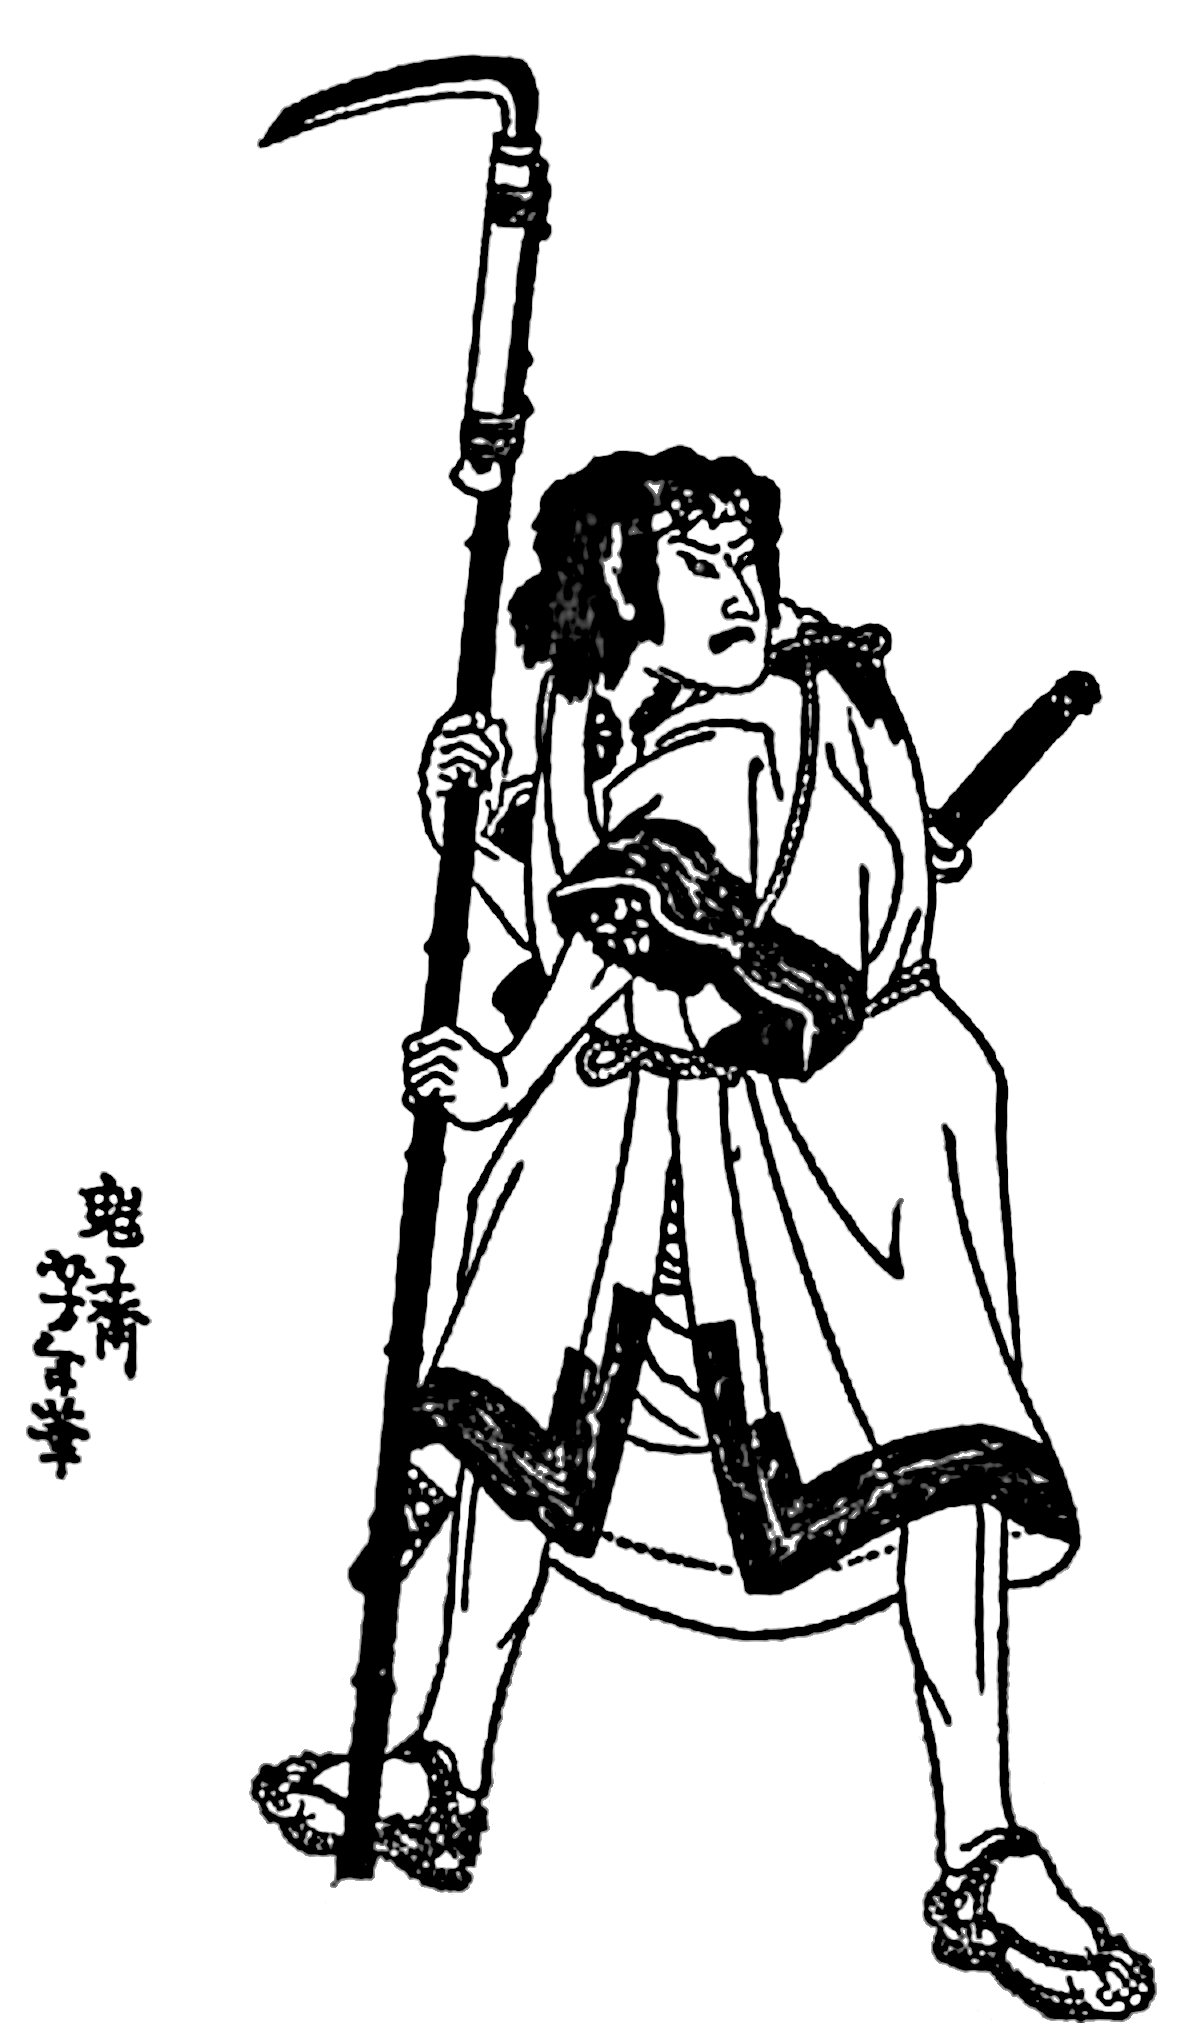
\includegraphics[width=60mm]{naigama}
\end{figure}

\vfill

\begin{table}[]
\centering
\begin{tabular}{ll}
Accompanies release & \input{../../../release} \\
Author &  Kees-Jan Hermans / kees.jan.hermans@gmail.com \\
Classification & - \\
Generated on & \today \\
\end{tabular}
\end{table}

% Accompanies release: \input{../../release}
% 
% Author: Kees-Jan Hermans / kees.jan.hermans@gmail.com
% 
% Classification: -
% 
% Generated on: \today
\newpage

\tableofcontents

\setlength{\parindent}{4em}
\setlength{\parskip}{1em}

\newpage
\section{Introduction}

\subsection{Parsing Expression Grammars}

This is the documentation describing Naigama, which is a collection of
specifications, libraries and tools enabling data parsing. It is based, by
now loosely, on Lua Parsing Expression Grammars, or LPEG [REF], which
implements a Packrat [REF] parsing algorithm.

\subsection{Naigama}

Naigama adds to Lua PEG the following features:

\begin{itemize}
\item Discoverability features:

  \begin{itemize}
  \item A fully fledges assembler step in between grammar and bytecode.
  \item A capable engine debugger.
  \end{itemize}

\item Extra tools:

  \begin{itemize}
  \item A disassembler.
  \item A decompiler.
  \end{itemize}

\item Security features:

  \begin{itemize}
  \item Bit upset event detection and traps.
  \item Endless loop detection.
  \end{itemize}

\item Interoperability with C (library, header files).
\item Added instructions for counters.
\item Added instructions for parsing binary inputs.
\item A scripting language.
\end{itemize}


\newpage
\section{Overview}

This document describes the Naigama parsing system, which is a 
modular system to process structured arbitrary length data inputs,
in order to extract meaning (matching, capturing from data), or to
manipulate (replacements within data).
The system was designed with a focus on information and system security.

The system comes in three parts: a grammar compiler, an assembler,
and a bytecode execution engine. Each of the parts has their own
input file format specification (grammar description, assembly specification,
and bytecode specification), and outputs the format of the next stage.
The process in brief: the compiler takes a
grammar description that the human end user has made, and turns it into
an assembly language. The assembler takes the assembly, and turns it
into a bytecode. The engine takes the bytecode and the input, and
processes it, resulting either in (various measures of) failure or
success.

%\begin{myquote}
%\begin{verbatim}
%Program:      _ Compiler       _  Assembler       _ Engine
%              /|         \     /|           \     /|  /|\  \
%             /           _\|  /             _\|  /     |   _\|
%Format: Grammar          Assembly           Bytecode   |   Output
%                                                       |
%                                                     Input
%\end{verbatim}
%\end{myquote}
%\textit{Schematic overview of Naigama data format transformation and modules}

\begin{center}
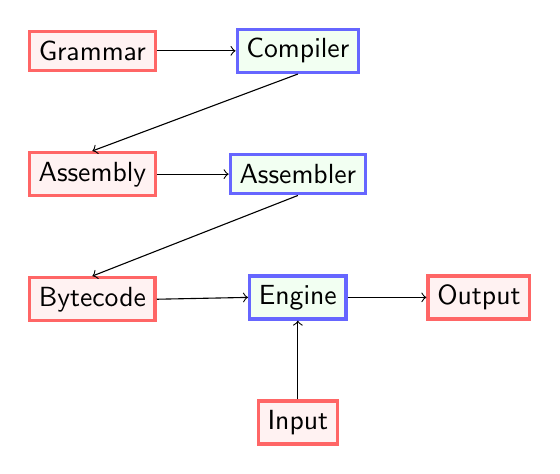
\begin{tikzpicture} [
bluenode/.style={rectangle, draw=blue!60, fill=green!5, very thick, minimum size=5mm},
rednode/.style={rectangle, draw=red!60, fill=red!5, very thick, minimum size=5mm},
]
%Nodes
\node[rednode]     (grammar)                            {Grammar};
\node[bluenode]    (compiler)    [right=of grammar]     {Compiler};
\node[rednode]     (assembly)    [below=of grammar]     {Assembly};
\node[bluenode]    (assembler)   [below=of compiler]    {Assembler};
\node[rednode]     (bytecode)    [below=of assembly]    {Bytecode};
\node[bluenode]    (engine)      [below=of assembler]   {Engine};
\node[rednode]     (input)       [below=of engine]      {Input};
\node[rednode]     (output)      [right=of engine]      {Output};

%Lines
\draw[->] (grammar.east) -- (compiler.west);
\draw[->] (compiler.south) -- (assembly.north);
\draw[->] (assembly.east) -- (assembler.west);
\draw[->] (assembler.south) -- (bytecode.north);
\draw[->] (bytecode.east) -- (engine.west);
\draw[->] (input.north) -- (engine.south);
\draw[->] (engine.east) -- (output.west);

\end{tikzpicture}

\textit{Schematic overview of Naigama data format transformation and tools}

\end{center}


The reason for this modularity is strict separation of tasks, and openness:
anyone should be able to take out a module, and replace it with one
of their own.
It should be expressly possible to take out the compiler, and replace
it with another tool that produces the Naigama assembly, for example.
Or have a different engine. Or write an optimizer for the assembly.

\subsection{On Grammar}
  
Naigama grammar is the human interface of the system.
It can be used to define complex syntax definitions in order
to match, capture from, and replace in, structured inputs.

People familiar with regular expressions \cite{bib:regex},
Backus-Naur syntax descriptions \cite{bib:backusnaur},
and / or Lex and Yacc tools \cite{bib:yacc},
should find this part of the document relatively easy to understand.
The ideas underlying Naigama grammar, assembly and bytecode
are heavily borrowed from Lua PEG (LPEG) \cite{bib:peg}
by Roberto Ierusalimschy et al.

\subsection{On Assembly}

The Naigama assembly language is a mixture of two languages:
For one, it is the outcome instruction set, according to the
aforementioned LPEG whitepaper,
of the Naigama grammar compilation process. However, it also contains
instructions that won't be produced by this compiler, but may
either be produced by a separate optimizer, or other compilers
altogether (for example, one that focuses on network packet
parsing).

The Naigama assembly language, in all cases, is the human readable
variant of the Naigama bytecode, and its instructions are one-on-one
translatable from the one to the other, and vice versa
(although labels will be lost in the reverse process).

\subsection{On Bytecode}

Naigama bytecode is the machine interface of the system.
It runs in the Naigama engine against the input provided by the user.
It is designed to be:

\begin{itemize}

\item Easy and quick to interpret.
\item Resilient against bit upset events.
\item Resilient against endless loops.
\item Usable while keeping both bytecode and input as read-only buffers.

\end{itemize}


\newpage
\section{Generations}

Naigama is written in generations. That is to say:
each subsequent generation of Naigama uses the tools generated
in the previous one, to build itself ('the grammar parses the grammar').

The following generations exist, with the following functions:

\begin{itemize}

\item Generation zero: This generation consists solely of a bootstrap
      grammar compiler and assembler written in perl.

\item Generation one: This generation is
      built in C, based on the bytecode to parse grammar grammar
      and assembly grammar, generated by generation zero.

\item Generation two: equal to generation one, but then based on
      the bytecode generated by the tooling in generation one.
      Generation two is 'pure' in that it has compiled itself,
      and it only provides parsing.

\item Generation three: this generation adds some concepts to the
      otherwise self-sufficient generation two (imports and
      isolation). It is this generation that does not yet enable
      scripting, but does diverge from Lua PEG completely.

\item Generation four: This generation extends the concept of the
      language further in that it also allows scripting.
      The parser of the scripting language is not 'active' however,
      because it's performed by generation two.
      It's equivalent to generation zero, in that it is the bootstrap
      compiler for scripting.

\item Generation five: This generation has the compiler and assembler
      defined as active scripts, including grammar. There is no
      support required for their execution, save for the engine's
      implementation in C.

\item Generation six: This generation is 'pure' again, in that it
      is equivalent to generation four, but then compiled by itself.

\end{itemize}


\newpage
\section{Grammar}
\label{sec:grammar}

A Naigama grammar file or buffer consists either of a single
unnamed expression, or of a sequence of named expressions (called rules),
whitespace and comments, denoted in ASCII text.
Naigama grammar is defined with the express purpose of matching, validating
and/or capturing from an arbitrary data input.
Naigama grammar is taken by the Naigama compiler program (naic) and turned
into Naigama assembly [section \ref{sec:assembly}].
In this, it resembles greatly other grammar description and parsing methods
such as Backus-Naur, Regular Expressions, Lex and Yacc.

\begin{myquote}
\begin{verbatim}
-- JSON; JavaScript Object Notation.
TOP          <- JSON
__prefix     <- %s*
JSON         <- HASH END
HASH         <- CBOPEN OPTHASHELTS CBCLOSE
OPTHASHELTS  <- HASHELTS / ...
HASHELTS     <- HASHELT COMMA HASHELTS / HASHELT
HASHELT      <- STRING COLON VALUE
ARRAY        <- ABOPEN OPTARRAYELTS ABCLOSE
OPTARRAYELTS <- ARRAYELTS / ...
ARRAYELTS    <- VALUE COMMA ARRAYELTS / VALUE
VALUE        <- STRING / FLOAT / INT / BOOL / NULL / HASH / ARRAY
STRING       <- { '"' ( '\\' ([nrtv"] / [0-9]^3) / [^"\\] )* '"' }
INT          <- { [0-9]+ }
FLOAT        <- { [0-9]* '.' [0-9]+ }
BOOL         <- { 'true' / 'false' }
NULL         <- { 'null' }
CBOPEN       <- '{'
CBCLOSE      <- '}'
ABOPEN       <- '['
ABCLOSE      <- ']'
COMMA        <- ','
COLON        <- ':'
END          <- !.
\end{verbatim}
\end{myquote}
\textit{Example of a Naigama grammar meant to validate and capture from
JSON\cite{bib:json} text.}

\subsection{Caveats}

This section highlights a few things to keep in mind when using
Naigama, or PEGs in general.

\subsubsection{Greedy and Blind Behavior}

PEG is, by itself, both greedy and blind.
That is to say, it consumes as much input as possible (greedy), and it does not
look ahead whether a next token is perhaps a better match for the input (blind).
It can however, also implement non-blind behavior, both in a greedy as
well as a non-greedy manner.

Having a greedy, blind parser - standard PEGs - implies that the following
rule will always fail (because the '.*' will consume all input):

\begin{myquote}
\begin{verbatim}
RULE <- .* 'foo'
\end{verbatim}
\end{myquote}

Grammars or patterns like the above, are usually treated in a more
friendly way by, for example, Regex parsers. They implement
a recursive algorithm around 'does the whole pattern match' question,
which backtracks 'from zero to any amount' quantifiers such as the one
used above,
leaving the user with a much more freedom to implement patterns but,
in the end, a much more unpredictable system (for example, what if
'foo' happens twice in the text?)

Naigama is not so understanding. To make it match something while
also doing a lookahead (therefore 'non blind'),
you can implement the following pattern
recursively (non greedy, so catching the first lookahead match):

\begin{myquote}
\begin{verbatim}
S <- E2 / E1 S
\end{verbatim}
\end{myquote}

Or, not recursively:

\begin{myquote}
\begin{verbatim}
S <- ( !E2 E1 )* E2
\end{verbatim}
\end{myquote}

And greedy, so catching only the last lookahead match:

\begin{myquote}
\begin{verbatim}
S <- E1 S / E2
\end{verbatim}
\end{myquote}

\subsubsection{Recursiveness}

Just like with greedy matching, Naigama will simply jump headlong
into your rule's first matcher, and will not try to second-guess your
intentions. So while in many grammar systems, left recursive is
usually considered the best way to describe
repetition, PEG will get stuck in an endless loop if you do the following:

\begin{myquote}
\begin{verbatim}
S <- S SOMEOTHER
\end{verbatim}
\end{myquote}

\subsection{Comments}

A comment starts with two minus signs and ends at the end of the line.

\begin{myquote}
\begin{verbatim}
-- Example of a single line comment.
\end{verbatim}
\end{myquote}

A multiline comment is also avaiable: these start with two minus signs
followed by two angle braces. The multiline comment is closed by two
closing angle braces.

\begin{myquote}
\begin{verbatim}
--[[
     Example of a
     multiline comment.
  ]]
\end{verbatim}
\end{myquote}

\subsection{Rules}

A rule is defined as an \textit{Identifier}, followed by a
left-pointing arrow (composed of a less-than and a minus sign),
followed by a matching expression.

When a Naigama grammar consists of a sequence of rules
(as opposed to a single line expression),
the first rule is used as the starting point for matching inputs.

\begin{myquote}
\begin{verbatim}
RULE1 <- 'a' / RULE2
RULE2 <- 'b' / RULE3
RULE3 <- 'c'
\end{verbatim}
\end{myquote}
\textit{Definition of a set of rules}

\subsubsection{Identifiers}

Identifiers, in Naigama, are defined as a combination of letters,
numbers and the underscore character, not starting with a number,
of between one and 64 characters long.

\begin{myquote}
\begin{verbatim}
IDENTIFIER <- [a-zA-Z_][a-zA-Z0-9_]^-63
\end{verbatim}
\end{myquote}

Identifiers are used to start rule definitions, and as references
to rules in expressions.

\subsubsection{Special Rules}

There is currently one special rule in Naigama grammar: a rule called
'\_\_prefix' will be treated specially. This rule will be, from its
definition onwards, called before the execution of any subsequent rule
definition expression. The aim is to make whitespace and comment filtering
in program language parsing easier. See also the earlier 'JSON' grammar
example.

\subsection{Expressions}

Expressions are lists of terms, optionally separated by the
OR operator (denoted by the forward slash sign).

\begin{myquote}
\begin{verbatim}
ALTERNATIVES <- ALT1 / ALT2 / ALT3
\end{verbatim}
\end{myquote}

A sequence of terms has a higher precendence than the OR operator,
so any other desired order of precedence has to be forced by using
brackets.
In the example below, the expressions evaluate differently:

\begin{myquote}
\begin{verbatim}
RULE1 <- 'a' 'b' / 'c'
RULE2 <- 'a' ( 'b' / 'c' )
\end{verbatim}
\end{myquote}

\subsection{Terms}

A term is defined as a matcher, potentially adorned with prefix
or postfix operators (though not at the same time).
Prefix operators are the NOT and CONFIRM modifiers.
Postfix operators are the quantifiers.

\subsubsection{The NOT Modifier}

The NOT modifier is an exclamation mark.
It does not advance the input position, but succeeds
when matching fails (including reaching the end of input),
and fails when matching succeeds.
Since Naigama is a greedy parser,
this can be used to implement a non-greedy lookahead, for example:
 
\begin{myquote}
\begin{verbatim}
CMULTILINECOMMENT <- '/*' (!'*/' .)* '*/'
\end{verbatim}
\end{myquote}

\subsubsection{The CONFIRM Modifier}

The CONFIRM modifier is an ampersand.
It does not advance the input position, and succeeds
as matching succeeds, and fails when matching fails.
It can be used to process (parts of the) input twice.
It is equivalent to using the NOT modifier twice.

Example where the input is first confirmed to be valid UTF-8,
and only after that, processed again from the beginning, for
well-formedness.
\begin{myquote}
\begin{verbatim}
JSON <- & UTF8 WELLFORMED
\end{verbatim}
\end{myquote}

\subsubsection{Quantifiers}

Naigama denotes quantifiers using a circonflex, followed by either
an absolute number, or a range. Shorthand exists for certain, often-used
ranges. These shorthand ranges are common in Regex as well:

\begin{center}
\caption{Naigama Quantifiers}
\label{tab:naig_quantifiers}
\begin{longtable}{ll}
\textbf{Quantifier} & \textbf{Semantics} \\
\endhead
* & Zero or more matches \\
+ & One or more matches \\
? & Zero or one matches \\
\^{}\textit{n} & \textit{n} matches \\
\^{}-\textit{n} & Zero up to and including \textit{n} matches \\
\^{}\textit{n}- & \textit{n} matches or more \\
\^{}\textit{n}-\textit{m} & From \textit{n} up to and including \textit{m} matches \\
\end{longtable}
\end{center}
 
Example of the use of quantifiers:
\begin{myquote}
\begin{verbatim}
RULE1 <- 'a'? 'b'^-5
\end{verbatim}
\end{myquote}

\subsection{Matchers}

\subsubsection{The ANY Matcher}

The ANY matcher is denoted (like in Regex) with a single dot.
It matches any character of input and it succeeds - advancing the input
pointer by one - if it can find one at the input pointer. It fails only
at the end of input.

\begin{myquote}
\begin{verbatim}
RUNGREEDILYTOTHEENDOFINPUT <- .*
\end{verbatim}
\end{myquote}

\subsubsection{The SET Matcher}

The ANY matcher, together with the NOT modifier,
also allows you to define end-of-input, like so:

\begin{myquote}
\begin{verbatim}
ENDOFINPUT <- !.
\end{verbatim}
\end{myquote}

\subsubsection{The SET Matcher}

The SET matcher is denoted, like in Regex, as a series of literals
and ranges, enclosed between angled brackets. It can also be negated,
in which case it matches any character not in the set.

\begin{myquote}
\begin{verbatim}
ALPHABETIC     <- [a-zA-Z]
NONALPHABETIC  <- [^a-zA-Z]
\end{verbatim}
\end{myquote}

The denotation of the set elements has a backslash as escape character
(to encode the minus and the closing angled brace).
It also has a form of binary escaping, to encode non-ASCII characters
as part of the set: a backslash followed by three digits of the characters
octal notation.

\subsubsection{The STRING Matcher}

The STRING matcher is denoted as a string literal, between single
quotes. The string may be postfixed with an lower case 'i' to
indicate (alphabetic) case insensitive matching.

\begin{myquote}
\begin{verbatim}
CASEINSENSTIVESTRING <- 'peg'i
\end{verbatim}
\end{myquote}

\subsubsection{The BITMASK Matcher}

The BITMASK matcher allows you to match bits.

\subsubsection{The HEXLITERAL Matcher}

The HEXLITERAL matcher allows you to match single characters by
through their hexadecimal representation.

\subsubsection{The MACRO Matcher}

All macroes are shorthand equivalents of the SET matcher.

\begin{center}
\caption{Naigama Macroes}
\label{tab:naig_macroes}
\begin{longtable}{lll}
\textbf{Macro} & \textbf{Semantics} & \textbf{Set} \\
\endhead
\%s & Whitespace & [ \textbackslash n\textbackslash r\textbackslash t\textbackslash v] \\
\%w & Alphabetic & [a-zA-Z] \\
\%a & Alphanumeric & [a-zA-Z0-9] \\
\%n & Numeric & [0-9] \\
\end{longtable}
\end{center}

\subsubsection{The GROUP Matcher}

\subsubsection{The CAPTURE Matcher}

\subsubsection{The VARCAPTURE Matcher}

\subsubsection{The VARREFERENCE Matcher}

\subsubsection{The REFERENCE Matcher}

\subsubsection{The LIMITEDINPUT Matcher}

\subsubsection{The END Matcher}



\newpage
\section{Assembly}
\label{sec:assembly}

A Naigama assembly file or buffer consists of sequences of
whitespace, comments, labels, and (parametrized) instructions, separated
by new lines, and denoted in ASCII text.

Naigama assembly is taken by the Naigama assembler program (naia) and turned
into bytecode.

\begin{myquote}
\begin{verbatim}
-- Compilation of: TEST <- { 'a' } { 'a' } { 'a' / 'b' }
  call TEST
  end
-- Rule
TEST:
  opencapture 0
  char 61
  closecapture 0 0
  opencapture 1
  char 61
  closecapture 1 0
  opencapture 2
  catch __LABEL_30 -- alternative
  char 61
  commit __LABEL_31
__LABEL_30:
  char 62
__LABEL_31:
  closecapture 2 0
  ret
\end{verbatim}
\end{myquote}
\textit{Example of a piece of Naigama assembly}

\subsection{Comments}

Just like in Naigama grammar,
comments in Naigama assembly start with two minus signs, and end at
a new line. They can be given on separate lines, or they can be
postfixed to instructions or labels.

\subsection{Labels}

Labels are identifiers (the same identifiers as in their definition
in the grammar chapter) or numbers, followed by a colon sign. They are used
as positions for the bytecode to jump to, when used by instructions.

When performing the assembly, the Naigama assembler program resolves
each label to their offset in the resultant bytecode, and replaces each
reference to a label with that offset.

Labels don't quite disappear though - you have the option to make the
assembler program emit a so called 'labelmap' file, which stores the old
label names, mapped to the bytecode offsets given by the assembler,
and which can be used later
for debugging purposes by the bytecode execution engine.

When disassembling (bytecode to assembly), each instruction is always
prefixed by a label in the form of the instruction's offset in decimal,
so that jumps are always correct (but non descriptive).

\subsubsection{Special Labels}

Certain instructions allow a special label called '\_\_NEXT\_\_' to be
used as parameter. Its function is to make instruction simply jump to
the next instruction on success.
This special label is there to avoid generating a special purpose label
only to put it right after the instruction using it.

The instructions allowing the use of the '\_\_NEXT\_\_' label are:

\begin{itemize}
\item backcommit
\item commit
\item condjump
\item partialcommit
\item testany
\item testchar
\item testquad
\item testset
\end{itemize}

\subsection{Instructions}


%\begin{table}[]
\begin{center}
\caption{Naigama Assembly Instructions}
\label{tab:naig_assembly}
\begin{longtable}{lll}
\textbf{Mnemonic} & \textbf{Param1} & \textbf{Param2} \\
\endhead
'any' &  &  \\
'backcommit' &  & LABEL \\
'call' &  & LABEL \\
'catch' &  & LABEL \\
'char' & char &  \\
'closecapture' & slot &  \\
'commit' &  & LABEL \\
'condjump' & register & LABEL \\
'counter' & register & value \\
'end' & code &  \\
'endisolate' &  &  \\
'endreplace' &  &  \\
'fail' &  &  \\
'failtwice' &  &  \\
'intrpcapture' &  &  \\
'isolate' & slot &  \\
'jump' &  & LABEL \\
'maskedchar' & char & mask \\
'noop' &  &  \\
'opencapture' & slot &  \\
'partialcommit' &  & LABEL \\
'quad' & quad &  \\
'range' & from & until \\
'replace' & slot & LABEL \\
'ret' &  &  \\
'set' & set &  \\
'skip' & number &  \\
'span' & set &  \\
'testany' &  & LABEL \\
'testchar' & char & LABEL \\
'testquad' & quad & LABEL \\
'testset' & set & LABEL \\
'trap' &  &  \\
'var' & slot &  \\
\end{longtable}
\end{center}
%\end{table}


See table [\ref{tab:naig_assembly}].

\subsection{Parameters}

Parameters follow the instruction in assembly text. They are separated
from the instruction and any other parameters by spaces. The following
types of parameters exist:

\subsubsection{Characters}

Character parameters are denoted as two byte hexadecimal values.

\subsubsection{Quads}

Quad parameters are denoted as eight byte hexadecimal values.

\subsubsection{Sets}

Set parameters are denoted as 64 byte hexadecimal values, representing
a bitmask of 256 possible booleans.

\subsubsection{Registers, Slots, Codes and Numbers}

These parameters are all denoted as decimal numbers.

\subsubsection{Caveats}

Note that the order of parameters sometimes reverses between the assembly
and bytecode specification. This is done because in assembly, it is
considered more aesthetically pleasing to have labels at the end of an
instruction, while in bytecode they are usually given as the first argument.

Consider, for example, the 'testchar' instruction, which in assembly is
given as:

\begin{myquote}
\begin{verbatim}
TESTCHARINSTR <- { 'testchar' } S HEXBYTE S LABEL
S <- %s+
HEXBYTE <- { [0-9a-fA-F]^2 }
LABEL <- { [a-zA-Z0-9_]^1-256 }
AMPERSAND <- '&'
\end{verbatim}
\end{myquote}

Whereas in bytecode, this instruction is encoded as:

%DEADBEEF
$_{00}$\ 
\fbox{%
  \parbox{20pt}{%
00
  }%
}
\fbox{%
  \parbox{20pt}{%
08
  }%
}
\fbox{%
  \parbox{20pt}{%
03
  }%
}
\fbox{%
  \parbox{20pt}{%
9a
  }%
}



$_{04}$\ 
\fbox{%
  \parbox{20pt}{%
00
  }%
}
\fbox{%
  \parbox{20pt}{%
00
  }%
}
\fbox{%
  \parbox{20pt}{%
00
  }%
}
\fbox{%
  \parbox{20pt}{%
00
  }%
}



$_{08}$\ 
\fbox{%
  \parbox{20pt}{%
00
  }%
}
\fbox{%
  \parbox{20pt}{%
00
  }%
}
\fbox{%
  \parbox{20pt}{%
00
  }%
}
\fbox{%
  \parbox{20pt}{%
00
  }%
}

Where:
  
Bytes 0-3 denote the instruction opcode.

Bytes 4-7 denote the bytecode offset to jump to, after
this instruction (big endian 32 bit unsigned).

Bytes 8-11 denote the character to match.


\newpage
\section{Bytecode}
\label{sec:bytecode}


%\begin{table}[]
\begin{center}
\caption{Naigama Bytecode Instructions}
\label{tab:naig_bytecode}
\begin{longtable}{lllll}
\textbf{Mnemonic} & \textbf{Opcode} & \textbf{Param1} & \textbf{Param2} & \textbf{Length} \\
\endhead
any & 000003e4 &  &   & 4 \\
backcommit & 000403c0 & address &   & 8 \\
call & 00040382 & address &   & 8 \\
catch & 00040393 & address &   & 8 \\
char & 000403d7 & char &   & 8 \\
closecapture & 00040300 & slot &   & 8 \\
commit & 00040336 & address &   & 8 \\
condjump & 00080321 & register & address  & 12 \\
counter & 00080356 & register & value  & 12 \\
end & 000400d8 & code &   & 8 \\
endisolate & 00003005 &  &   & 4 \\
endreplace & 00000399 &  &   & 4 \\
fail & 0000034b &  &   & 4 \\
failtwice & 00000390 &  &   & 4 \\
intrpcapture & 0008000f &  &   & 12 \\
isolate & 00043003 & slot &   & 8 \\
jump & 00040333 & address &   & 8 \\
maskedchar & 00080365 & char & mask  & 12 \\
mode & 0004000a &  &   & 8 \\
noop & 00000000 &  &   & 4 \\
opencapture & 0004039c & slot &   & 8 \\
partialcommit & 000403b4 & address &   & 8 \\
quad & 0004037e & quad &   & 8 \\
range & 000803bd & from & until  & 12 \\
replace & 00080348 & slot & address  & 12 \\
ret & 000003a0 &  &   & 4 \\
scr\_add & 0000050c &  &   & 4 \\
scr\_array & 00040006 &  &   & 8 \\
scr\_assign & 000005c9 &  &   & 4 \\
scr\_bitand & 00000527 &  &   & 4 \\
scr\_bitnot & 00000574 &  &   & 4 \\
scr\_bitor & 0000053c &  &   & 4 \\
scr\_bitxor & 0000052d &  &   & 4 \\
scr\_builtin & 000407cf &  &   & 8 \\
scr\_call & 00040503 &  &   & 8 \\
scr\_condjump & 0004000c &  &   & 8 \\
scr\_dec & 0000053a &  &   & 4 \\
scr\_div & 00000581 &  &   & 4 \\
scr\_equals & 0000056c &  &   & 4 \\
scr\_gt & 0000056f &  &   & 4 \\
scr\_gteq & 0000054d &  &   & 4 \\
scr\_inc & 000005f6 &  &   & 4 \\
scr\_index & 00000009 &  &   & 4 \\
scr\_logand & 0000052e &  &   & 4 \\
scr\_lognot & 000005f9 &  &   & 4 \\
scr\_logor & 000005a9 &  &   & 4 \\
scr\_lt & 00000595 &  &   & 4 \\
scr\_lteq & 00000522 &  &   & 4 \\
scr\_mul & 0000058b &  &   & 4 \\
scr\_nequals & 00000572 &  &   & 4 \\
scr\_pop & 000005cc &  &   & 4 \\
scr\_pow & 00000542 &  &   & 4 \\
scr\_push & 000c0003 &  &   & 16 \\
scr\_ret & 00000555 &  &   & 4 \\
scr\_shift & 00040005 &  &   & 8 \\
scr\_shiftin & 0000057d &  &   & 4 \\
scr\_shiftout & 00000517 &  &   & 4 \\
scr\_string & 000017bb &  &   & 4 \\
scr\_sub & 000005bb &  &   & 4 \\
set & 002003ca & set &   & 36 \\
skip & 00040330 & number &   & 8 \\
span & 002003e1 & set &   & 36 \\
testany & 00040306 & address &   & 8 \\
testchar & 0008039a & address & char  & 12 \\
testquad & 000803db & address & quad  & 12 \\
testset & 00240363 & address & set  & 40 \\
trap & ff00ffff &  &   & 4 \\
var & 000403ee & slot &   & 8 \\
\end{longtable}
\end{center}
%\end{table}


\subsection{Bytecode Structure}

A Naigama bytecode file or buffer consists of a sequence of binary
instructions which, in turn, each consist of a binary
encoded opcode, plus their parameters, should they have any.

The amount and kind of parameters following an opcode, is strictly
defined:
the same opcode will always be followed by the same kinds of parameters
and therefore, an instruction type will always be the same size
(see table [\ref{tab:naig_bytecode}]).

Naigama bytecode is taken by the Naigama engine program (naie) or
library, and run against an input, to produce an output.

\subsection{Opcode Values}

Opcode values are determined through

\begin{itemize}
\item Grouping; 
\item Hamming distance;
\item Instruction size;
\end{itemize}

\subsection{Noop Slides and Canaries}

Implementations that want each instruction to have exactly the
same size, can choose to pad the encoding of shorter instructions
with either no-ops, or canaries.

\subsection{Encoding of Parameters}

\subsubsection{Address}

\subsubsection{Char}

\subsubsection{Slot}

\subsubsection{Register}


\newpage
\section{Output}


\newpage
\section{Executables}

\subsection{The Compiler}

The Naigama grammar compiler is called 'naic'.
It takes a grammar file as input, and outputs assembly text.
It can be invoked as follows:

\begin{myquote}
\begin{verbatim}
$ naic -i myfile.niag -o myfile.asm
\end{verbatim}
\end{myquote}
\textit{Example of the invocation of the Naigama grammar compiler}

Bear in mind that both the input (grammar) file, as well as the
output (assembly) file may be omitted (in which case they will be
assumed to be stdin and stdout, respectively), or be denoted as
a minus sign ('-'), which will have the same effect.

You may also use the following options:

\begin{itemize}
\item \texttt{-m $<$path$>$} Tells the compiler to emit the slotmap
      file in $<$path$>$.
\item \texttt{-D} Creates a lot of debugging output.
\item \texttt{-t} Tells the compiler to surround generated rule
      code with 'trap' instructions.
\end{itemize}

\subsection{The Assembler}

The Naigama grammar assember is called 'naia'.
It takes an assembly file as input, and outputs bytecode.
It can be invoked as follows:

\begin{myquote}
\begin{verbatim}
$ naia -i myfile.asm -o myfile.byc
\end{verbatim}
\end{myquote}
\textit{Example of the invocation of the Naigama assembler}

Bear in mind that both the input (assembly) file, as well as the
output (bytecode) file may be omitted (in which case they will be
assumed to be stdin and stdout, respectively), or be denoted as
a minus sign ('-'), which will have the same effect.

You may also use the following options:

\begin{itemize}
\item \texttt{-l $<$path$>$} Tells the assembler to emit the labelmap
      file in $<$path$>$.
\item \texttt{-D} Creates a lot of debugging output.
\end{itemize}

\subsection{The Engine}

The Naigama bytecode execution engine is called 'naie'.
It takes a bytecode file as input, as well as an input file.
It can be invoked as follows:

\begin{myquote}
\begin{verbatim}
$ naie -c myfile.byc -i myfile.dat -o myfile.out
\end{verbatim}
\end{myquote}
\textit{Example of the invocation of the Naigama engine}

\subsection{The Disassembler}

The Naigama disassembler is called 'naid'.
It takes a bytecode file as input, and outputs assembly.

\begin{myquote}
\begin{verbatim}
$ naid -i myfile.byc -o myfile.asm
\end{verbatim}
\end{myquote}
\textit{Example of the invocation of the Naigama disassembler}

The output of the disassembler will differ from the assembly
generated by the compiler in that:

\begin{itemize}
\item Textual labels will be gone, instead:
\item Every instruction will be prefixed by a numeric label which
      is identical to that instruction's position offset in the bytecode, and
\item All jumps will therefore also be using those position labels.
\end{itemize}


\newpage
\section{File Formats}

This section describes all the user available memory and file formats
associated with Naigama.

\subsection{Text Formats}

\subsubsection{Grammar}

The Naigama grammar text format is descibed in [REF].
Various pre-compilers can potentially produce these format however,
these are out of scope of this documentation. The grammar format is
consumed by the Naigama assembler, naic. For the use of naic, see [REF].

\subsubsection{Assembly}

The Naigama assembly text format is descibed in [REF].
This format is produced by the Naigama compiler, naic,
and is consumed by the Naigama assembler, naia.
For the use of naia, see [REF].

\subsubsection{Slotmap.h}

The Naigama compiler assigns a slot number to each capture it encounters.
It then assigns an internal unique name to those capture numbers, or slots.
Finally, the compiler can be requested, through the command line, to
'rain down' these named mappings to slot number in a C-header file, so that
API users can use easy-to-remember #defines to address their captures.

\subsubsection{Disassembly}

The Naigama disassembler, naid, will take bytecode and reproduce the
assembly. This assembly will be different from the original assembly
in that:

\begin{itemize}
\item It will not contain textually understandable labels.
\item It will prefix every instruction with a numeric label, which is
      equivalent to the bytecode offset of the instruction's opcode.
\item These offsets will then also be used in jumps.
\end{itemize}

\subsubsection{Engine Debug Logs}

Running the Naigama engine, naie, in debug mode will yield, on standard error,
a log, which will contain, per instruction executed, a line representing
the engine's internal state, most notably its stack, like so:

\begin{myquote}
\begin{verbatim}
CHAR bc 2316 in 482 0403020100______ st (014 prec.) ALT:1484
CLL:1476 C LL:1820 ALT:1944 CLL:1928 ALT:1652 CLL:1644 CLL:2440
\end{verbatim}
\end{myquote}

These lines are built up as follows:

\begin{itemize}
\item The instruction being executed (in this case, 'char').
\item The bytecode offset (in this case, 2316 decimal).
\item The input offset (in this case, 482 decimal).
\item A subset of the input, from the input offset (in this in hexadecimal).
\item An overview of the stack (in this case, with 14 preceding items left
      out), followed by the last stack items, either 'call' items
      (with their return addresses), or 'alternative' items
      (with their jump-to addresses in case they catch a FAIL condition).
\end{itemize}

\subsection{Binary Formats}

This section describes the formats used by the Naigama tooling, other than
the ones described in the sections on grammar, assembly and bytecode.

\subsubsection{Slotmap Format}

The slotmap file exists to help developers by easing access to
captures in complex grammars.

The Naigama grammar compiler can be instructed to emit a slotmap file.
This is a file which maps a unique name to a capture region's index.
This is provided so that, instead of using the index of capture region
(which requires hand counting them in your grammar file, which can be
tedious and error-prone, and something that would not survive
a grammar reshuffle, or the introduction of a capture region before
the one you're interested in), you can use a naming scheme for your
capture regions.

Names in the slotmap file are bound semantically to the capture region:
they are made up of the name of the rule,
an underscore, and all alphabetic characters in the capture region,
cast to uppercase. Should any name occur twice, it will be postfixed with
a counter until it's unique.

For example, the following rule with capture region definition:

\begin{myquote}
\begin{verbatim}
RULE <- { IDENT } OPTARGS LEFTARROW EXPRESSION
\end{verbatim}
\end{myquote}

will result in slotmap identifier 'RULE\_IDENT'.

The binary format of a slotmap file is composed as a sequence of binary records:
the slot index, denoted as a 32 bit network order unsigned integer, a
field of 32 bit all ones, and the slot name, denoted as a zero-terminated
string.

\begin{myquote}
\begin{verbatim}
00 00 00 00 ff ff ff ff 52 55 4c 45 5f 49 44 45  ........RULE_IDE
4e 54 00 00 00 00 01 ff ff ff ff 45 58 50 52 45  NT.........EXPRE
53 53 49 4f 4e 5f 54 45 52 4d 53 00 00 00 00 02  SSION_TERMS.....
ff ff ff ff 45 58 50 52 45 53 53 49 4f 4e 5f 54  ....EXPRESSION_T
45 52 4d 53 5f 31 00 00 00 00 03 ff ff ff ff 45  ERMS_1.........E
58 50 52 45 53 53 49 4f 4e 5f 54 45 52 4d 53 5f  XPRESSION_TERMS_
32 00 00 00 00 04 ff ff ff ff 54 45 52 4d 53 5f  2.........TERMS_
54 45 52 4d 00 00 00 00 05 ff ff ff ff 54 45 52  TERM.........TER
4d 5f 4e 4f 54 41 4e 44 00 00 00 00 06 ff ff ff  M_NOTAND........
\end{verbatim}
\end{myquote}
\textit{Example of the head of a slotmap file, hex dumped}

\subsubsection{Labelmap Format}

The labelmap format is optionally emitted by the assembler, and exists to:

\begin{itemize}
\item Allow for better debugging, because offsets in bytecode can be reduced
      to more intuitively named sections (rule names always make it to
      the labelmap unchanged).
\item Allow for calling the bytecode at symbols directly, which in turn
      allows you to use a bytecode blob more as a database of functions.
\end{itemize}

The binary format of the labelmap file is composed as a sequence of
binary records: the bytecode offset, denoted as a 32 bit network order
unsigned integer, followed by the labelstring, followed by a zero byte.

\begin{myquote}
\begin{verbatim}
00 00 00 10 47 52 41 4d 4d 41 52 00 00 00 00 28  ....GRAMMAR....(
5f 5f 4c 41 42 45 4c 5f 31 31 00 00 00 00 38 5f  __LABEL_11....8_
5f 4c 41 42 45 4c 5f 31 32 00 00 00 00 40 5f 5f  _LABEL_12....@__
4c 41 42 45 4c 5f 36 00 00 00 00 48 5f 5f 4c 41  LABEL_6....H__LA
42 45 4c 5f 37 00 00 00 00 54 5f 5f 70 72 65 66  BEL_7....T__pref
69 78 00 00 00 00 5c 5f 5f 4c 41 42 45 4c 5f 32  ix....\__LABEL_2
39 00 00 00 00 7c 5f 5f 4c 41 42 45 4c 5f 34 33  9....|__LABEL_43
00 00 00 00 a8 5f 5f 4c 41 42 45 4c 5f 34 34 00  .....__LABEL_44.
00 00 00 b8 5f 5f 4c 41 42 45 4c 5f 33 32 00 00  ....__LABEL_32..
00 00 e4 5f 5f 4c 41 42 45 4c 5f 35 35 00 00 00  ...__LABEL_55...
01 10 5f 5f 4c 41 42 45 4c 5f 35 36 00 00 00 01  ..__LABEL_56....
10 5f 5f 4c 41 42 45 4c 5f 33 33 00 00 00 01 18  .__LABEL_33.....
5f 5f 4c 41 42 45 4c 5f 33 30 00 00 00 01 1c 45  __LABEL_30.....E
4e 44 00 00 00 01 34 5f 5f 4c 41 42 45 4c 5f 35  ND....4__LABEL_5
38 00 00 00 01 38 44 45 46 49 4e 49 54 49 4f 4e  8....8DEFINITION
00 00 00 01 4c 53 49 4e 47 4c 45 5f 45 58 50 52  ....LSINGLE_EXPR
45 53 53 49 4f 4e 00 00 00 01 60 52 55 4c 45 00  ESSION....`RULE.
00 00 01 a0 45 58 50 52 45 53 53 49 4f 4e 00 00  ....EXPRESSION..
00 01 e4 5f 5f 4c 41 42 45 4c 5f 31 30 36 00 00  ...__LABEL_106..
\end{verbatim}
\end{myquote}
\textit{Example of a section of labelmap file, hex dumped}

\subsubsection{Engine Output Format}

The Naigama bytecode execution engine, naie, produces, on success, output for
digital processing, in the form of a binary table, which is structured
as follows:

\begin{itemize}

\item Each record is four 32 bit integers, in network order.

\item The first record contains the end code of the matching process.
This is the same code as was given as a parameter to the 'end'
instruction that resulted in the execution finishing. This is the
first field, by default it is zero.
The second field contains the amount of subsequent records.

\item Subsequent records have as fields, either:

\begin{itemize}
\item Type, slot, start, length (when of 'capture' type), or:
\item Type, slot, start, char (when of 'replace' type).
\end{itemize}

\end{itemize}

Bear in mind the following:

\begin{itemize}
\item 'Capture' type is denoted as 1, 'Replace' as 3.
\item Offsets and lengths of captures refer to the input buffer.
\item Offsets and lengths of replacements refer to the bytecode.
\end{itemize}

\begin{myquote}
\begin{verbatim}
00 00 00 00 00 00 03 64 00 00 00 00 00 00 00 00  .......d........
00 00 00 01 00 00 00 00 00 00 00 1c 00 00 00 23  ...............#
00 00 00 01 00 00 00 03 00 00 00 32 00 00 00 59  ...........2...Y
00 00 00 01 00 00 00 04 00 00 00 32 00 00 00 55  ...........2...U
00 00 00 01 00 00 00 14 00 00 00 32 00 00 00 55  ...........2...U
00 00 00 01 00 00 00 02 00 00 00 34 00 00 00 3f  ...........4...?
00 00 00 01 00 00 00 04 00 00 00 34 00 00 00 3f  ...........4...?
00 00 00 01 00 00 00 17 00 00 00 34 00 00 00 3e  ...........4...>
00 00 00 01 00 00 00 06 00 00 00 3e 00 00 00 3f  ...........>...?
00 00 00 01 00 00 00 03 00 00 00 42 00 00 00 53  ...........B...S
00 00 00 01 00 00 00 04 00 00 00 42 00 00 00 53  ...........B...S
00 00 00 01 00 00 00 17 00 00 00 42 00 00 00 53  ...........B...S
\end{verbatim}
\end{myquote}
\textit{Example of the head of engine output with a zero end code
and 868 matches (all captures), hex dumped}


\newpage
\section{API's}

\subsection{Languages}

\subsection{C API Concepts}

\subsubsection{Main Structures}

\subsubsection{Error Handling}

Naigama C library function prototypes are (almost) all typed to return
the NAIG\_ERR\_T type.

\subsection{Compiler}

\subsection{Assembler}

\subsection{Engine}

\subsection{All in one API}

The compound API provides an interface to all of the action in one place.

\subsubsection{Includes}

\begin{myquote}
\begin{verbatim}
#include <naigama/naigama.h>
\end{verbatim}
\end{myquote}

\subsubsection{Initialization}

\subsubsection{Using the parser}

\begin{myquote}
\begin{verbatim}
NAIG_ERR_T naig_compile
  (naig_t* naig, char* grammar, int traps);
\end{verbatim}
\end{myquote}

\begin{myquote}
\begin{verbatim}
NAIG_ERR_T naig_run
  (
    naig_t*         naig,
    unsigned char*  input,
    unsigned        input_length,
    naio_result_t*  result
  );
\end{verbatim}
\end{myquote}

\subsubsection{Using the Result Structure}

To include the proper types and functions, use:

\begin{myquote}
\begin{verbatim}
#include <naigama/memio/naio.h>
\end{verbatim}
\end{myquote}

The definition of the associated types:

\begin{myquote}
\begin{verbatim}
typedef struct {
  uint32_t              action;
  uint32_t              slot;
  uint32_t              start;
  uint32_t              length; // dubs as char/quad in replace
}
naio_resact_t;

typedef struct
{
  int                   code;
  naio_resact_t*        actions;
  unsigned              length; // allocated
  unsigned              count;  // used
}
naio_result_t;
\end{verbatim}
\end{myquote}

You can step through each action (up to result-$>$count),
and for each result-$>$actions[ i ], check its action
(which can be one of NAIG\_ACTION\_OPENCAPTURE,
NAIG\_ACTION\_DELETE, NAIG\_ACTION\_REPLACE\_CHAR, or
NAIG\_ACTION\_REPLACE\_QUAD),
its slot number (this will be the iterator that the compiler uses
for each encountered capture region), and its start and length.
You'll still need the input buffer handy, because this type does
not provide you with the capture data itself.

If you're only interested in capturing, then you'll only
need the NAIG\_ACTION\_OPENCAPTURE action type. Also when
your grammar does not contain any replacement definitions, you'll never
encounter any other action type in the capture list.

\subsubsection{Performing Replacements}

...

\subsubsection{Getting a Malloced Capture Tree}

To handle capture data independently of the input buffer, and
preprocessed to represent a capture tree, you can use the following API:

\begin{myquote}
\begin{verbatim}
extern
naio_resobj_t* naio_result_object
  (
    const unsigned char*  input,
    unsigned              inputlength,
    naio_result_t*        result
  )
  __attribute__ ((warn_unused_result));
\end{verbatim}
\end{myquote}

\begin{myquote}
\begin{verbatim}
struct naio_resobj
{
  unsigned              type;
  char*                 string;
  unsigned              stringlen;
  unsigned              origoffset;
  naio_resobj_t*        parent;
  naio_resobj_t**       children;
  unsigned              nchildren;
  unsigned              slotnumber;
  void*                 auxptr; /* this one is for you */
};
\end{verbatim}
\end{myquote}

Below is a simplified version of the naio\_result\_object\_debug function,
which shows you how you can recursively step through your capture
list and print an indented capture result tree.

\begin{myquote}
\begin{verbatim}
void naio_result_object_debug
  (naio_resobj_t* object, unsigned indent)
{
  unsigned i;

  if ((int)(object->type) == -1) {
    fprintf(stderr, "TOP  - ");
  } else {
    fprintf(stderr, "%.4u ", object->type);
  }
  for (i=0; i < indent; i++) {
    fprintf(stderr, "--");
  }
  fprintf(stderr, "| %s\n", object->string);
  for (i=0; i < object->nchildren; i++) {
    naio_result_object_debug(object->children[ i ], indent + 1);
  }
}
\end{verbatim}
\end{myquote}



\newpage
\section{Colofon}
\listoftables
\begin{thebibliography}{12}

\bibitem{bib:peg}
  A Text Pattern-Matching Tool based on Parsing Expression Grammars
  https://www.inf.puc-rio.br/\textasciitilde roberto/docs/peg.pdf

\bibitem{bib:regex}
  Regular Expressions
  https://en.wikipedia.org/wiki/Regular\_expression

\bibitem{bib:backusnaur}
  Backus Naur Form
  https://en.wikipedia.org/wiki/Backus-Naur\_form

\bibitem{bib:yacc}
  Yacc Yet Another Compiler Compiler
  https://en.wikipedia.org/wiki/Yacc

\bibitem{bib:javascript}
  JavaScript, or ECMAScript
  https://www.ecma-international.org/publications/standards/Ecma-262.htm

\bibitem{bib:json}
  JSON, JavaScript Object Notation
  https://www.json.org/

\bibitem{bib:perl}
  Perl, the Perl Programming Language
  https://www.perl.org/

\end{thebibliography}


\newpage
\begin{appendices}

\section{Instructions}
\label{app:instr}

This appendix treats all Naigama (assembly / bytecode) instructions,
plus the FAIL event (which eats up the execution stack up to and
including the highest 'catch' element).


%DEADBEEF
\newpage
\subsection{Instruction: any}

\subsubsection{Summary}

The 'any' instruction checks to see if there is a character of input
left to consume, and consumes it if there is. Otherwise it causes a failure.

\subsubsection{Grammar and Compiling}

The '.' (dot) matcher used in grammar, like in regular expressions
\cite{bib:regex}, means 'match any character'. In Perl \cite{bib:perl}
a modifier has to be added to make it include matching of newlines.
In Naigama, 'any character' is confined to 8-bit characters (bytes).

\subsubsection{Assembly Syntax}

\begin{myquote}
\begin{verbatim}
ANYINSTR <- 'any'

\end{verbatim}
\end{myquote}

\subsubsection{Bytecode Encoding}

This instruction is structured in bytecode as follows:

%DEADBEEF
$_0$\ 
\fbox{%
  \parbox{20pt}{%
00
  }%
}
\fbox{%
  \parbox{20pt}{%
00
  }%
}
\fbox{%
  \parbox{20pt}{%
03
  }%
}
\fbox{%
  \parbox{20pt}{%
21
  }%
}

%DEADBEEF
\subsubsection{Execution State Change}

.

Original state: \textit{(p, i, e, c)}

Operation: \textbf{any} ; i \ \textless \ $\vert$S$\vert$

Failure state: \textit{(\textbf{Fail}, i, e, c)}

Success state: \textit{(p + 1, i + 1, e, c)}



\newpage
\subsection{Instruction: backcommit}

\subsubsection{Mode}
This instruction is available in mode 0 (parser).
\subsubsection{Summary}

\InputIfFileExists{instr_backcommit_summary.tex}{}{}

\subsubsection{Grammar and Compiling}

\InputIfFileExists{instr_backcommit_compiling.tex}{}{}

\subsubsection{Assembly Syntax}

\begin{myquote}
\begin{verbatim}
BACKCOMMITINSTR <- { 'backcommit' } S LABEL
S <- %s+
LABEL <- { [a-zA-Z0-9_]^1-64 }
\end{verbatim}
\end{myquote}

\subsubsection{Bytecode Encoding}

This instruction has a size of 8 bytes and is structured in bytecode as follows:

%DEADBEEF
$_{00}$\ 
\fbox{%
  \parbox{20pt}{%
00
  }%
}
\fbox{%
  \parbox{20pt}{%
04
  }%
}
\fbox{%
  \parbox{20pt}{%
03
  }%
}
\fbox{%
  \parbox{20pt}{%
c0
  }%
}



$_{04}$\ 
\fbox{%
  \parbox{20pt}{%
00
  }%
}
\fbox{%
  \parbox{20pt}{%
00
  }%
}
\fbox{%
  \parbox{20pt}{%
00
  }%
}
\fbox{%
  \parbox{20pt}{%
00
  }%
}

%DEADBEEF
\subsubsection{Execution State Change}

.

\InputIfFileExists{instr_backcommit_state.tex}{}{}



\newpage
\subsection{Instruction: call}

\subsubsection{Mode}
This instruction is available in mode 0 (parser).
\subsubsection{Summary}

\InputIfFileExists{instr_call_summary.tex}{}{}

\subsubsection{Grammar and Compiling}

\InputIfFileExists{instr_call_compiling.tex}{}{}

\subsubsection{Assembly Syntax}

\begin{myquote}
\begin{verbatim}
CALLINSTR <- { 'call' } S LABEL
S <- %s+
LABEL <- { [a-zA-Z0-9_]^1-64 }
\end{verbatim}
\end{myquote}

\subsubsection{Bytecode Encoding}

This instruction has a size of 8 bytes and is structured in bytecode as follows:

%DEADBEEF
$_{00}$\ 
\fbox{%
  \parbox{20pt}{%
00
  }%
}
\fbox{%
  \parbox{20pt}{%
04
  }%
}
\fbox{%
  \parbox{20pt}{%
03
  }%
}
\fbox{%
  \parbox{20pt}{%
82
  }%
}



$_{04}$\ 
\fbox{%
  \parbox{20pt}{%
00
  }%
}
\fbox{%
  \parbox{20pt}{%
00
  }%
}
\fbox{%
  \parbox{20pt}{%
00
  }%
}
\fbox{%
  \parbox{20pt}{%
00
  }%
}

%DEADBEEF
\subsubsection{Execution State Change}

.

\InputIfFileExists{instr_call_state.tex}{}{}



\newpage
\subsection{Instruction: catch}

\subsubsection{Summary}

The 'catch' instruction pushes a 'catch' element on the stack,
in which the current state of the engine is captured (input position,
height of the action list), as well as a bytecode offset, which
is where the engine jumps to when the element is popped due to a FAIL
condition.

\subsubsection{Grammar and Compiling}

Several constructs in the Naigama grammar emit a 'catch' instruction,
for example:

\begin{itemize}

\item A 'choice' situation, which is when an OR operator ('/', or
slash forward) is introduced in an expression.

\item A 'not' situation, which is when a matcher is prefixed with a NOT
operator ('!', or exclamation mark).

\item A 'not-not' situation, which is when a matcher is prefixed with an
ampersand ('\&').

\item A quantifier on a matcher that is forgiving, for example allowing
infinite repetitions of a matcher, or values between a minimum and a
maximum.

\end{itemize}

\subsubsection{Assembly Syntax}

\begin{myquote}
\begin{verbatim}
CATCHINSTR <- 'catch' S LABEL
S          <- %s+
LABEL      <- [a-zA-Z0-9_]^1-64

\end{verbatim}
\end{myquote}

\subsubsection{Bytecode Encoding}

This instruction is structured in bytecode as follows:

%DEADBEEF
$_0$\ 
\fbox{%
  \parbox{20pt}{%
00
  }%
}
\fbox{%
  \parbox{20pt}{%
04
  }%
}
\fbox{%
  \parbox{20pt}{%
0a
  }%
}
\fbox{%
  \parbox{20pt}{%
03
  }%
}

%DEADBEEF

$_4$\
\fbox{%
  \parbox{20pt}{%
nn
  }%
}
\fbox{%
  \parbox{20pt}{%
nn
  }%
}
\fbox{%
  \parbox{20pt}{%
nn
  }%
}
\fbox{%
  \parbox{20pt}{%
nn
  }%
}

Where 'nn' is a 32-bit, network encoded, valid bytecode offset.

\subsubsection{Execution State Change}

.

Original state: \textit{(p, i, e, c)}

Operation: \textbf{catch n}

Failure state: -

Success state: \textit{(p + 1, i, e:(n,p,i), c)}



\newpage
\subsection{Instruction: char}

\subsubsection{Summary}

The 'char' instruction compares its only parameter, a character value,
against the character value at the current input offset. If they are
equal, the match is considered a success, and the engine moves to the
next instruction. If they are not equal, the FAIL condition is raised.

\subsubsection{Grammar and Compiling}

In grammar, the 'char' instruction is emitted by the compiler from
the treatment of a string literal.

\subsubsection{Assembly Syntax}

\begin{myquote}
\begin{verbatim}
CHARINSTR <- 'char' S HEXBYTE
S         <- %s+
HEXBYTE   <- [0-9a-fA-F]^2

\end{verbatim}
\end{myquote}
\subsubsection{Bytecode Encoding}

This instruction is structured in bytecode as follows:

%DEADBEEF
$_0$\ 
\fbox{%
  \parbox{20pt}{%
00
  }%
}
\fbox{%
  \parbox{20pt}{%
04
  }%
}
\fbox{%
  \parbox{20pt}{%
05
  }%
}
\fbox{%
  \parbox{20pt}{%
09
  }%
}

%DEADBEEF

$_4$\
\fbox{%
  \parbox{20pt}{%
nn
  }%
}
\fbox{%
  \parbox{20pt}{%
nn
  }%
}
\fbox{%
  \parbox{20pt}{%
nn
  }%
}
\fbox{%
  \parbox{20pt}{%
nn
  }%
}

Where 'nn' is a 32-bit, network encoded, character value.

\subsubsection{Execution State Change}

.

Original state: \textit{(p, i, e, c)}

Operation: \textbf{char c}

Failure state: \textit{(\textbf{Fail}, i, e, c)}

Success state: \textit{(p + 1, i + 1, e, c)}



\newpage
\subsection{Instruction: closecapture}

\subsubsection{Mode}
This instruction is available in mode 0 (parser).
\subsubsection{Summary}

\InputIfFileExists{instr_closecapture_summary.tex}{}{}

\subsubsection{Grammar and Compiling}

\InputIfFileExists{instr_closecapture_compiling.tex}{}{}

\subsubsection{Assembly Syntax}

\begin{myquote}
\begin{verbatim}
CLOSECAPTUREINSTR <- { 'closecapture' } S SLOT ( S TYPE )?
S <- %s+
SLOT <- UNSIGNED
TYPE <- UNSIGNED
\end{verbatim}
\end{myquote}

\subsubsection{Bytecode Encoding}

This instruction has a size of 8 bytes and is structured in bytecode as follows:

%DEADBEEF
$_{00}$\ 
\fbox{%
  \parbox{20pt}{%
00
  }%
}
\fbox{%
  \parbox{20pt}{%
04
  }%
}
\fbox{%
  \parbox{20pt}{%
03
  }%
}
\fbox{%
  \parbox{20pt}{%
00
  }%
}



$_{04}$\ 
\fbox{%
  \parbox{20pt}{%
00
  }%
}
\fbox{%
  \parbox{20pt}{%
00
  }%
}
\fbox{%
  \parbox{20pt}{%
00
  }%
}
\fbox{%
  \parbox{20pt}{%
00
  }%
}

%DEADBEEF
\subsubsection{Execution State Change}

.

\InputIfFileExists{instr_closecapture_state.tex}{}{}



\newpage
\subsection{Instruction: commit}

\subsubsection{Summary}

\InputIfFileExists{instr_commit_summary.tex}{}{}

\subsubsection{Grammar and Compiling}

\InputIfFileExists{instr_commit_compiling.tex}{}{}

\subsubsection{Assembly Syntax}

\begin{myquote}
\begin{verbatim}
COMMITINSTR <- { 'commit' } S LABEL
S <- %s+
LABEL <- { [a-zA-Z0-9_]^1-256 }
\end{verbatim}
\end{myquote}

\subsubsection{Bytecode Encoding}

This instruction has a size of 8 bytes and is structured in bytecode as follows:

%DEADBEEF
$_{00}$\ 
\fbox{%
  \parbox{20pt}{%
00
  }%
}
\fbox{%
  \parbox{20pt}{%
04
  }%
}
\fbox{%
  \parbox{20pt}{%
03
  }%
}
\fbox{%
  \parbox{20pt}{%
36
  }%
}



$_{04}$\ 
\fbox{%
  \parbox{20pt}{%
00
  }%
}
\fbox{%
  \parbox{20pt}{%
00
  }%
}
\fbox{%
  \parbox{20pt}{%
00
  }%
}
\fbox{%
  \parbox{20pt}{%
00
  }%
}

%DEADBEEF
\InputIfFileExists{instr_commit_bytecode.tex}{}{}

\subsubsection{Execution State Change}

.

\InputIfFileExists{instr_commit_state.tex}{}{}



\newpage
\subsection{Instruction: condjump}

\subsubsection{Summary}

\InputIfFileExists{instr_condjump_summary.tex}{}{}

\subsubsection{Grammar and Compiling}

\InputIfFileExists{instr_condjump_compiling.tex}{}{}

\subsubsection{Assembly Syntax}

\begin{myquote}
\begin{verbatim}
CONDJUMPINSTR <- { 'condjump' } S REGISTER S LABEL
S <- %s+
REGISTER <- UNSIGNED
LABEL <- { [a-zA-Z0-9_]^1-64 }
\end{verbatim}
\end{myquote}

\InputIfFileExists{instr_condjump_assembly.tex}{}{}

\subsubsection{Bytecode Encoding}

This instruction has a size of 12 bytes and is structured in bytecode as follows:

%DEADBEEF
$_{00}$\ 
\fbox{%
  \parbox{20pt}{%
00
  }%
}
\fbox{%
  \parbox{20pt}{%
08
  }%
}
\fbox{%
  \parbox{20pt}{%
03
  }%
}
\fbox{%
  \parbox{20pt}{%
21
  }%
}



$_{04}$\ 
\fbox{%
  \parbox{20pt}{%
00
  }%
}
\fbox{%
  \parbox{20pt}{%
00
  }%
}
\fbox{%
  \parbox{20pt}{%
00
  }%
}
\fbox{%
  \parbox{20pt}{%
00
  }%
}



$_{08}$\ 
\fbox{%
  \parbox{20pt}{%
00
  }%
}
\fbox{%
  \parbox{20pt}{%
00
  }%
}
\fbox{%
  \parbox{20pt}{%
00
  }%
}
\fbox{%
  \parbox{20pt}{%
00
  }%
}

%DEADBEEF
\InputIfFileExists{instr_condjump_bytecode.tex}{}{}

\subsubsection{Execution State Change}

.

\InputIfFileExists{instr_condjump_state.tex}{}{}



\newpage
\subsection{Instruction: counter}

\subsubsection{Summary}

\InputIfFileExists{instr_counter_summary.tex}{}{}

\subsubsection{Grammar and Compiling}

\InputIfFileExists{instr_counter_compiling.tex}{}{}

\subsubsection{Assembly Syntax}

\begin{myquote}
\begin{verbatim}
COUNTERINSTR <- { 'counter' } S REGISTER S UNSIGNED
S <- %s+
REGISTER <- UNSIGNED
UNSIGNED <- { [0-9]+ }
\end{verbatim}
\end{myquote}

\subsubsection{Bytecode Encoding}

This instruction has a size of 12 bytes and is structured in bytecode as follows:

%DEADBEEF
$_{00}$\ 
\fbox{%
  \parbox{20pt}{%
00
  }%
}
\fbox{%
  \parbox{20pt}{%
08
  }%
}
\fbox{%
  \parbox{20pt}{%
03
  }%
}
\fbox{%
  \parbox{20pt}{%
56
  }%
}



$_{04}$\ 
\fbox{%
  \parbox{20pt}{%
00
  }%
}
\fbox{%
  \parbox{20pt}{%
00
  }%
}
\fbox{%
  \parbox{20pt}{%
00
  }%
}
\fbox{%
  \parbox{20pt}{%
00
  }%
}



$_{08}$\ 
\fbox{%
  \parbox{20pt}{%
00
  }%
}
\fbox{%
  \parbox{20pt}{%
00
  }%
}
\fbox{%
  \parbox{20pt}{%
00
  }%
}
\fbox{%
  \parbox{20pt}{%
00
  }%
}

%DEADBEEF
\InputIfFileExists{instr_counter_bytecode.tex}{}{}

\subsubsection{Execution State Change}

.

\InputIfFileExists{instr_counter_state.tex}{}{}



\newpage
\subsection{Instruction: end}

\subsubsection{Summary}

\InputIfFileExists{instr_end_summary.tex}{}{}

\subsubsection{Grammar and Compiling}

\InputIfFileExists{instr_end_compiling.tex}{}{}

\subsubsection{Assembly Syntax}

\begin{myquote}
\begin{verbatim}
ENDINSTR <- { 'end' } S CODE
S <- %s+
CODE <- UNSIGNED
\end{verbatim}
\end{myquote}

\InputIfFileExists{instr_end_assembly.tex}{}{}

\subsubsection{Bytecode Encoding}

This instruction has a size of 8 bytes and is structured in bytecode as follows:

%DEADBEEF
$_{00}$\ 
\fbox{%
  \parbox{20pt}{%
00
  }%
}
\fbox{%
  \parbox{20pt}{%
04
  }%
}
\fbox{%
  \parbox{20pt}{%
00
  }%
}
\fbox{%
  \parbox{20pt}{%
d8
  }%
}



$_{04}$\ 
\fbox{%
  \parbox{20pt}{%
00
  }%
}
\fbox{%
  \parbox{20pt}{%
00
  }%
}
\fbox{%
  \parbox{20pt}{%
00
  }%
}
\fbox{%
  \parbox{20pt}{%
00
  }%
}

%DEADBEEF
\InputIfFileExists{instr_end_bytecode.tex}{}{}

\subsubsection{Execution State Change}

.

\InputIfFileExists{instr_end_state.tex}{}{}



\newpage
\subsection{Instruction: endreplace}

\subsubsection{Mode}
This instruction is available in mode 0 (parser).
\subsubsection{Summary}

\InputIfFileExists{instr_endreplace_summary.tex}{}{}

\subsubsection{Grammar and Compiling}

\InputIfFileExists{instr_endreplace_compiling.tex}{}{}

\subsubsection{Assembly Syntax}

\begin{myquote}
\begin{verbatim}
ENDREPLACEINSTR <- { 'endreplace' }
\end{verbatim}
\end{myquote}

\subsubsection{Bytecode Encoding}

This instruction has a size of 4 bytes and is structured in bytecode as follows:

%DEADBEEF
$_{00}$\ 
\fbox{%
  \parbox{20pt}{%
00
  }%
}
\fbox{%
  \parbox{20pt}{%
00
  }%
}
\fbox{%
  \parbox{20pt}{%
03
  }%
}
\fbox{%
  \parbox{20pt}{%
99
  }%
}

%DEADBEEF
\InputIfFileExists{instr_endreplace_bytecode.tex}{}{}

\subsubsection{Execution State Change}

.

\InputIfFileExists{instr_endreplace_state.tex}{}{}



\newpage
\subsection{Instruction: fail}

\subsubsection{Summary}

\InputIfFileExists{instr_fail_summary.tex}{}{}

\subsubsection{Grammar and Compiling}

\InputIfFileExists{instr_fail_compiling.tex}{}{}

\subsubsection{Assembly Syntax}

\begin{myquote}
\begin{verbatim}
FAILINSTR <- { 'fail' }
\end{verbatim}
\end{myquote}

\InputIfFileExists{instr_fail_assembly.tex}{}{}

\subsubsection{Bytecode Encoding}

This instruction has a size of 4 bytes and is structured in bytecode as follows:

%DEADBEEF
$_{00}$\ 
\fbox{%
  \parbox{20pt}{%
00
  }%
}
\fbox{%
  \parbox{20pt}{%
00
  }%
}
\fbox{%
  \parbox{20pt}{%
03
  }%
}
\fbox{%
  \parbox{20pt}{%
4b
  }%
}

%DEADBEEF
\InputIfFileExists{instr_fail_bytecode.tex}{}{}

\subsubsection{Execution State Change}

.

\InputIfFileExists{instr_fail_state.tex}{}{}



\newpage
\subsection{Instruction: failtwice}

\subsubsection{Mode}
This instruction is available in mode 0 (parser).
\subsubsection{Summary}

\InputIfFileExists{instr_failtwice_summary.tex}{}{}

\subsubsection{Grammar and Compiling}

\InputIfFileExists{instr_failtwice_compiling.tex}{}{}

\subsubsection{Assembly Syntax}

\begin{myquote}
\begin{verbatim}
FAILTWICEINSTR <- { 'failtwice' }
\end{verbatim}
\end{myquote}

\subsubsection{Bytecode Encoding}

This instruction has a size of 4 bytes and is structured in bytecode as follows:

%DEADBEEF
$_{00}$\ 
\fbox{%
  \parbox{20pt}{%
00
  }%
}
\fbox{%
  \parbox{20pt}{%
00
  }%
}
\fbox{%
  \parbox{20pt}{%
03
  }%
}
\fbox{%
  \parbox{20pt}{%
90
  }%
}

%DEADBEEF
\subsubsection{Execution State Change}

.

\InputIfFileExists{instr_failtwice_state.tex}{}{}



\newpage
\subsection{Instruction: jump}

\subsubsection{Mode}
This instruction is available in both mode 0 (parser) and mode 1 (script interpreter).
\subsubsection{Summary}

\InputIfFileExists{instr_jump_summary.tex}{}{}

\subsubsection{Grammar and Compiling}

\InputIfFileExists{instr_jump_compiling.tex}{}{}

\subsubsection{Assembly Syntax}

\begin{myquote}
\begin{verbatim}
JUMPINSTR <- { 'jump' } S LABEL
S <- %s+
LABEL <- { [a-zA-Z0-9_]^1-64 }
\end{verbatim}
\end{myquote}

\subsubsection{Bytecode Encoding}

This instruction has a size of 8 bytes and is structured in bytecode as follows:

%DEADBEEF
$_{00}$\ 
\fbox{%
  \parbox{20pt}{%
00
  }%
}
\fbox{%
  \parbox{20pt}{%
04
  }%
}
\fbox{%
  \parbox{20pt}{%
03
  }%
}
\fbox{%
  \parbox{20pt}{%
33
  }%
}



$_{04}$\ 
\fbox{%
  \parbox{20pt}{%
00
  }%
}
\fbox{%
  \parbox{20pt}{%
00
  }%
}
\fbox{%
  \parbox{20pt}{%
00
  }%
}
\fbox{%
  \parbox{20pt}{%
00
  }%
}

%DEADBEEF
\subsubsection{Execution State Change}

.

\InputIfFileExists{instr_jump_state.tex}{}{}



\newpage
\subsection{Instruction: maskedchar}

\subsubsection{Mode}
This instruction is available in mode 0 (parser).
\subsubsection{Summary}

\InputIfFileExists{instr_maskedchar_summary.tex}{}{}

\subsubsection{Grammar and Compiling}

\InputIfFileExists{instr_maskedchar_compiling.tex}{}{}

\subsubsection{Assembly Syntax}

\begin{myquote}
\begin{verbatim}
MASKEDCHARINSTR <- { 'maskedchar' } S HEXBYTE S HEXBYTE
S <- %s+
HEXBYTE <- { [0-9a-fA-F]^2 }
\end{verbatim}
\end{myquote}

\subsubsection{Bytecode Encoding}

This instruction has a size of 12 bytes and is structured in bytecode as follows:

%DEADBEEF
$_{00}$\ 
\fbox{%
  \parbox{20pt}{%
00
  }%
}
\fbox{%
  \parbox{20pt}{%
08
  }%
}
\fbox{%
  \parbox{20pt}{%
03
  }%
}
\fbox{%
  \parbox{20pt}{%
65
  }%
}



$_{04}$\ 
\fbox{%
  \parbox{20pt}{%
00
  }%
}
\fbox{%
  \parbox{20pt}{%
00
  }%
}
\fbox{%
  \parbox{20pt}{%
00
  }%
}
\fbox{%
  \parbox{20pt}{%
00
  }%
}



$_{08}$\ 
\fbox{%
  \parbox{20pt}{%
00
  }%
}
\fbox{%
  \parbox{20pt}{%
00
  }%
}
\fbox{%
  \parbox{20pt}{%
00
  }%
}
\fbox{%
  \parbox{20pt}{%
00
  }%
}

%DEADBEEF
\InputIfFileExists{instr_maskedchar_bytecode.tex}{}{}

\subsubsection{Execution State Change}

.

\InputIfFileExists{instr_maskedchar_state.tex}{}{}



\newpage
\subsection{Instruction: noop}

\subsubsection{Mode}
This instruction is available in both mode 0 (parser) and mode 1 (script interpreter).
\subsubsection{Summary}

\InputIfFileExists{instr_noop_summary.tex}{}{}

\subsubsection{Grammar and Compiling}

\InputIfFileExists{instr_noop_compiling.tex}{}{}

\subsubsection{Assembly Syntax}

\begin{myquote}
\begin{verbatim}
NOOPINSTR <- { 'noop' }
\end{verbatim}
\end{myquote}

\subsubsection{Bytecode Encoding}

This instruction has a size of 4 bytes and is structured in bytecode as follows:

%DEADBEEF
$_{00}$\ 
\fbox{%
  \parbox{20pt}{%
00
  }%
}
\fbox{%
  \parbox{20pt}{%
00
  }%
}
\fbox{%
  \parbox{20pt}{%
00
  }%
}
\fbox{%
  \parbox{20pt}{%
00
  }%
}

%DEADBEEF
\InputIfFileExists{instr_noop_bytecode.tex}{}{}

\subsubsection{Execution State Change}

.

\InputIfFileExists{instr_noop_state.tex}{}{}



\newpage
\subsection{Instruction: opencapture}

\subsubsection{Mode}
This instruction is available in mode 0 (parser).
\subsubsection{Summary}

\InputIfFileExists{instr_opencapture_summary.tex}{}{}

\subsubsection{Grammar and Compiling}

\InputIfFileExists{instr_opencapture_compiling.tex}{}{}

\subsubsection{Assembly Syntax}

\begin{myquote}
\begin{verbatim}
OPENCAPTUREINSTR <- { 'opencapture' } S SLOT
S <- %s+
SLOT <- UNSIGNED
\end{verbatim}
\end{myquote}

\subsubsection{Bytecode Encoding}

This instruction has a size of 8 bytes and is structured in bytecode as follows:

%DEADBEEF
$_{00}$\ 
\fbox{%
  \parbox{20pt}{%
00
  }%
}
\fbox{%
  \parbox{20pt}{%
04
  }%
}
\fbox{%
  \parbox{20pt}{%
03
  }%
}
\fbox{%
  \parbox{20pt}{%
9c
  }%
}



$_{04}$\ 
\fbox{%
  \parbox{20pt}{%
00
  }%
}
\fbox{%
  \parbox{20pt}{%
00
  }%
}
\fbox{%
  \parbox{20pt}{%
00
  }%
}
\fbox{%
  \parbox{20pt}{%
00
  }%
}

%DEADBEEF
\subsubsection{Execution State Change}

.

\InputIfFileExists{instr_opencapture_state.tex}{}{}



\newpage
\subsection{Instruction: partialcommit}

\subsubsection{Summary}

\InputIfFileExists{instr_partialcommit_summary.tex}{}{}

\subsubsection{Grammar and Compiling}

\InputIfFileExists{instr_partialcommit_compiling.tex}{}{}

\subsubsection{Assembly Syntax}

\begin{myquote}
\begin{verbatim}
PARTIALCOMMITINSTR <- { 'partialcommit' } S LABEL
S <- %s+
LABEL <- { [a-zA-Z0-9_]^1-256 }
\end{verbatim}
\end{myquote}

\subsubsection{Bytecode Encoding}

This instruction has a size of 8 bytes and is structured in bytecode as follows:

%DEADBEEF
$_{00}$\ 
\fbox{%
  \parbox{20pt}{%
00
  }%
}
\fbox{%
  \parbox{20pt}{%
04
  }%
}
\fbox{%
  \parbox{20pt}{%
03
  }%
}
\fbox{%
  \parbox{20pt}{%
b4
  }%
}



$_{04}$\ 
\fbox{%
  \parbox{20pt}{%
00
  }%
}
\fbox{%
  \parbox{20pt}{%
00
  }%
}
\fbox{%
  \parbox{20pt}{%
00
  }%
}
\fbox{%
  \parbox{20pt}{%
00
  }%
}

%DEADBEEF
\InputIfFileExists{instr_partialcommit_bytecode.tex}{}{}

\subsubsection{Execution State Change}

.

\InputIfFileExists{instr_partialcommit_state.tex}{}{}



\newpage
\subsection{Instruction: quad}

\subsubsection{Summary}

\subsubsection{Grammar and Compiling}

\subsubsection{Assembly Syntax}

\begin{myquote}
\begin{verbatim}

\end{verbatim}
\end{myquote}
\subsubsection{Bytecode Encoding}

This instruction is structured in bytecode as follows:

%DEADBEEF
$_0$\ 
\fbox{%
  \parbox{20pt}{%
00
  }%
}
\fbox{%
  \parbox{20pt}{%
04
  }%
}
\fbox{%
  \parbox{20pt}{%
03
  }%
}
\fbox{%
  \parbox{20pt}{%
09
  }%
}

%DEADBEEF
\subsubsection{Execution State Change}

.

Original state: \textit{(p, i, e, c)}

Operation: \textbf{any} ; i \ \textless \ $\vert$S$\vert$

Failure state: \textit{(\textbf{Fail}, i, e, c)}

Success state: \textit{(p + 1, i + 1, e, c)}



\newpage
\subsection{Instruction: range}

\subsubsection{Mode}
This instruction is available in mode 0 (parser).
\subsubsection{Summary}

\InputIfFileExists{instr_range_summary.tex}{}{}

\subsubsection{Grammar and Compiling}

\InputIfFileExists{instr_range_compiling.tex}{}{}

\subsubsection{Assembly Syntax}

\begin{myquote}
\begin{verbatim}
RANGEINSTR <- { 'range' } S UNSIGNED S UNSIGNED
S <- %s+
UNSIGNED <- { [0-9]+ }
\end{verbatim}
\end{myquote}

\subsubsection{Bytecode Encoding}

This instruction has a size of 12 bytes and is structured in bytecode as follows:

%DEADBEEF
$_{00}$\ 
\fbox{%
  \parbox{20pt}{%
00
  }%
}
\fbox{%
  \parbox{20pt}{%
08
  }%
}
\fbox{%
  \parbox{20pt}{%
03
  }%
}
\fbox{%
  \parbox{20pt}{%
bd
  }%
}



$_{04}$\ 
\fbox{%
  \parbox{20pt}{%
00
  }%
}
\fbox{%
  \parbox{20pt}{%
00
  }%
}
\fbox{%
  \parbox{20pt}{%
00
  }%
}
\fbox{%
  \parbox{20pt}{%
00
  }%
}



$_{08}$\ 
\fbox{%
  \parbox{20pt}{%
00
  }%
}
\fbox{%
  \parbox{20pt}{%
00
  }%
}
\fbox{%
  \parbox{20pt}{%
00
  }%
}
\fbox{%
  \parbox{20pt}{%
00
  }%
}

%DEADBEEF
\subsubsection{Execution State Change}

.

\InputIfFileExists{instr_range_state.tex}{}{}



\newpage
\subsection{Instruction: replace}

\subsubsection{Mode}
This instruction is available in mode 0 (parser).
\subsubsection{Summary}

\InputIfFileExists{instr_replace_summary.tex}{}{}

\subsubsection{Grammar and Compiling}

\InputIfFileExists{instr_replace_compiling.tex}{}{}

\subsubsection{Assembly Syntax}

\begin{myquote}
\begin{verbatim}
REPLACEINSTR <- { 'replace' } S SLOT S LABEL
S <- %s+
SLOT <- UNSIGNED
LABEL <- { [a-zA-Z0-9_]^1-64 }
\end{verbatim}
\end{myquote}

\subsubsection{Bytecode Encoding}

This instruction has a size of 12 bytes and is structured in bytecode as follows:

%DEADBEEF
$_{00}$\ 
\fbox{%
  \parbox{20pt}{%
00
  }%
}
\fbox{%
  \parbox{20pt}{%
08
  }%
}
\fbox{%
  \parbox{20pt}{%
03
  }%
}
\fbox{%
  \parbox{20pt}{%
48
  }%
}



$_{04}$\ 
\fbox{%
  \parbox{20pt}{%
00
  }%
}
\fbox{%
  \parbox{20pt}{%
00
  }%
}
\fbox{%
  \parbox{20pt}{%
00
  }%
}
\fbox{%
  \parbox{20pt}{%
00
  }%
}



$_{08}$\ 
\fbox{%
  \parbox{20pt}{%
00
  }%
}
\fbox{%
  \parbox{20pt}{%
00
  }%
}
\fbox{%
  \parbox{20pt}{%
00
  }%
}
\fbox{%
  \parbox{20pt}{%
00
  }%
}

%DEADBEEF
\InputIfFileExists{instr_replace_bytecode.tex}{}{}

\subsubsection{Execution State Change}

.

\InputIfFileExists{instr_replace_state.tex}{}{}



\newpage
\subsection{Instruction: ret}

\subsubsection{Summary}

\subsubsection{Grammar and Compiling}

\subsubsection{Assembly Syntax}

\begin{myquote}
\begin{verbatim}

\end{verbatim}
\end{myquote}
\subsubsection{Bytecode Encoding}

This instruction is structured in bytecode as follows:

%DEADBEEF
$_0$\ 
\fbox{%
  \parbox{20pt}{%
00
  }%
}
\fbox{%
  \parbox{20pt}{%
00
  }%
}
\fbox{%
  \parbox{20pt}{%
03
  }%
}
\fbox{%
  \parbox{20pt}{%
05
  }%
}

%DEADBEEF
\subsubsection{Execution State Change}

.

Original state: \textit{(p, i, e, c)}

Operation: \textbf{any} ; i \ \textless \ $\vert$S$\vert$

Failure state: \textit{(\textbf{Fail}, i, e, c)}

Success state: \textit{(p + 1, i + 1, e, c)}



\newpage
\subsection{Instruction: set}

\subsubsection{Summary}

\subsubsection{Grammar and Compiling}

\subsubsection{Assembly Syntax}

\begin{myquote}
\begin{verbatim}

\end{verbatim}
\end{myquote}
\subsubsection{Bytecode Encoding}

This instruction is structured in bytecode as follows:

%DEADBEEF
$_0$\ 
\fbox{%
  \parbox{20pt}{%
00
  }%
}
\fbox{%
  \parbox{20pt}{%
20
  }%
}
\fbox{%
  \parbox{20pt}{%
03
  }%
}
\fbox{%
  \parbox{20pt}{%
f9
  }%
}

%DEADBEEF
\subsubsection{Execution State Change}

.

Original state: \textit{(p, i, e, c)}

Operation: \textbf{any} ; i \ \textless \ $\vert$S$\vert$

Failure state: \textit{(\textbf{Fail}, i, e, c)}

Success state: \textit{(p + 1, i + 1, e, c)}



\newpage
\subsection{Instruction: skip}

\subsubsection{Summary}

\subsubsection{Grammar and Compiling}

\subsubsection{Assembly Syntax}

\begin{myquote}
\begin{verbatim}

\end{verbatim}
\end{myquote}
\subsubsection{Bytecode Encoding}

This instruction is structured in bytecode as follows:

%DEADBEEF
$_0$\ 
\fbox{%
  \parbox{20pt}{%
00
  }%
}
\fbox{%
  \parbox{20pt}{%
04
  }%
}
\fbox{%
  \parbox{20pt}{%
05
  }%
}
\fbox{%
  \parbox{20pt}{%
55
  }%
}

%DEADBEEF
\subsubsection{Execution State Change}

.

Original state: \textit{(p, i, e, c)}

Operation: \textbf{any} ; i \ \textless \ $\vert$S$\vert$

Failure state: \textit{(\textbf{Fail}, i, e, c)}

Success state: \textit{(p + 1, i + 1, e, c)}



\newpage
\subsection{Instruction: span}

\subsubsection{Summary}

\subsubsection{Grammar and Compiling}

\subsubsection{Assembly Syntax}

\begin{myquote}
\begin{verbatim}

\end{verbatim}
\end{myquote}
\subsubsection{Bytecode Encoding}

This instruction is structured in bytecode as follows:

%DEADBEEF
$_0$\ 
\fbox{%
  \parbox{20pt}{%
00
  }%
}
\fbox{%
  \parbox{20pt}{%
20
  }%
}
\fbox{%
  \parbox{20pt}{%
03
  }%
}
\fbox{%
  \parbox{20pt}{%
84
  }%
}

%DEADBEEF
\subsubsection{Execution State Change}

.

Original state: \textit{(p, i, e, c)}

Operation: \textbf{any} ; i \ \textless \ $\vert$S$\vert$

Failure state: \textit{(\textbf{Fail}, i, e, c)}

Success state: \textit{(p + 1, i + 1, e, c)}



\newpage
\subsection{Instruction: testany}

\subsubsection{Summary}

\InputIfFileExists{instr_testany_summary.tex}{}{}

\subsubsection{Grammar and Compiling}

\InputIfFileExists{instr_testany_compiling.tex}{}{}

\subsubsection{Assembly Syntax}

\begin{myquote}
\begin{verbatim}
TESTANYINSTR <- { 'testany' } S LABEL
S <- %s+
LABEL <- { [a-zA-Z0-9_]^1-64 }
\end{verbatim}
\end{myquote}

\subsubsection{Bytecode Encoding}

This instruction has a size of 8 bytes and is structured in bytecode as follows:

%DEADBEEF
$_{00}$\ 
\fbox{%
  \parbox{20pt}{%
00
  }%
}
\fbox{%
  \parbox{20pt}{%
04
  }%
}
\fbox{%
  \parbox{20pt}{%
03
  }%
}
\fbox{%
  \parbox{20pt}{%
06
  }%
}



$_{04}$\ 
\fbox{%
  \parbox{20pt}{%
00
  }%
}
\fbox{%
  \parbox{20pt}{%
00
  }%
}
\fbox{%
  \parbox{20pt}{%
00
  }%
}
\fbox{%
  \parbox{20pt}{%
00
  }%
}

%DEADBEEF
\InputIfFileExists{instr_testany_bytecode.tex}{}{}

\subsubsection{Execution State Change}

.

\InputIfFileExists{instr_testany_state.tex}{}{}



\newpage
\subsection{Instruction: testchar}

\subsubsection{Summary}

\InputIfFileExists{instr_testchar_summary.tex}{}{}

\subsubsection{Grammar and Compiling}

\InputIfFileExists{instr_testchar_compiling.tex}{}{}

\subsubsection{Assembly Syntax}

\begin{myquote}
\begin{verbatim}
TESTCHARINSTR <- { 'testchar' } S HEXBYTE S LABEL ( S AMPERSAND HEXBYTE )?
S <- %s+
HEXBYTE <- { [0-9a-fA-F]^2 }
LABEL <- { [a-zA-Z0-9_]^1-256 }
AMPERSAND <- '&'
\end{verbatim}
\end{myquote}

\subsubsection{Bytecode Encoding}

This instruction has a size of 12 bytes and is structured in bytecode as follows:

%DEADBEEF
$_{00}$\ 
\fbox{%
  \parbox{20pt}{%
00
  }%
}
\fbox{%
  \parbox{20pt}{%
08
  }%
}
\fbox{%
  \parbox{20pt}{%
03
  }%
}
\fbox{%
  \parbox{20pt}{%
9a
  }%
}



$_{04}$\ 
\fbox{%
  \parbox{20pt}{%
00
  }%
}
\fbox{%
  \parbox{20pt}{%
00
  }%
}
\fbox{%
  \parbox{20pt}{%
00
  }%
}
\fbox{%
  \parbox{20pt}{%
00
  }%
}



$_{08}$\ 
\fbox{%
  \parbox{20pt}{%
00
  }%
}
\fbox{%
  \parbox{20pt}{%
00
  }%
}
\fbox{%
  \parbox{20pt}{%
00
  }%
}
\fbox{%
  \parbox{20pt}{%
00
  }%
}

%DEADBEEF
\InputIfFileExists{instr_testchar_bytecode.tex}{}{}

\subsubsection{Execution State Change}

.

\InputIfFileExists{instr_testchar_state.tex}{}{}



\newpage
\subsection{Instruction: testquad}

\subsubsection{Summary}

\InputIfFileExists{instr_testquad_summary.tex}{}{}

\subsubsection{Grammar and Compiling}

\InputIfFileExists{instr_testquad_compiling.tex}{}{}

\subsubsection{Assembly Syntax}

\begin{myquote}
\begin{verbatim}
TESTQUADINSTR <- { 'testquad' } S QUAD S LABEL
S <- %s+
QUAD <- { [0-9a-fA-F]^8 }
LABEL <- { [a-zA-Z0-9_]^1-64 }
\end{verbatim}
\end{myquote}

\InputIfFileExists{instr_testquad_assembly.tex}{}{}

\subsubsection{Bytecode Encoding}

This instruction has a size of 12 bytes and is structured in bytecode as follows:

%DEADBEEF
$_{00}$\ 
\fbox{%
  \parbox{20pt}{%
00
  }%
}
\fbox{%
  \parbox{20pt}{%
08
  }%
}
\fbox{%
  \parbox{20pt}{%
03
  }%
}
\fbox{%
  \parbox{20pt}{%
db
  }%
}



$_{04}$\ 
\fbox{%
  \parbox{20pt}{%
00
  }%
}
\fbox{%
  \parbox{20pt}{%
00
  }%
}
\fbox{%
  \parbox{20pt}{%
00
  }%
}
\fbox{%
  \parbox{20pt}{%
00
  }%
}



$_{08}$\ 
\fbox{%
  \parbox{20pt}{%
00
  }%
}
\fbox{%
  \parbox{20pt}{%
00
  }%
}
\fbox{%
  \parbox{20pt}{%
00
  }%
}
\fbox{%
  \parbox{20pt}{%
00
  }%
}

%DEADBEEF
\InputIfFileExists{instr_testquad_bytecode.tex}{}{}

\subsubsection{Execution State Change}

.

\InputIfFileExists{instr_testquad_state.tex}{}{}



\newpage
\subsection{Instruction: testset}

\subsubsection{Summary}

\InputIfFileExists{instr_testset_summary.tex}{}{}

\subsubsection{Grammar and Compiling}

\InputIfFileExists{instr_testset_compiling.tex}{}{}

\subsubsection{Assembly Syntax}

\begin{myquote}
\begin{verbatim}
TESTSETINSTR <- { 'testset' } S SET S LABEL
S <- %s+
SET <- { [0-9a-fA-F]^64 }
LABEL <- { [a-zA-Z0-9_]^1-64 }
\end{verbatim}
\end{myquote}

\subsubsection{Bytecode Encoding}

This instruction has a size of 40 bytes and is structured in bytecode as follows:

%DEADBEEF
$_{00}$\ 
\fbox{%
  \parbox{20pt}{%
00
  }%
}
\fbox{%
  \parbox{20pt}{%
24
  }%
}
\fbox{%
  \parbox{20pt}{%
03
  }%
}
\fbox{%
  \parbox{20pt}{%
63
  }%
}



$_{04}$\ 
\fbox{%
  \parbox{20pt}{%
00
  }%
}
\fbox{%
  \parbox{20pt}{%
00
  }%
}
\fbox{%
  \parbox{20pt}{%
00
  }%
}
\fbox{%
  \parbox{20pt}{%
00
  }%
}



$_{08}$\ 
\fbox{%
  \parbox{20pt}{%
00
  }%
}
\fbox{%
  \parbox{20pt}{%
00
  }%
}
\fbox{%
  \parbox{20pt}{%
00
  }%
}
\fbox{%
  \parbox{20pt}{%
00
  }%
}



$_{12}$\ 
\fbox{%
  \parbox{20pt}{%
00
  }%
}
\fbox{%
  \parbox{20pt}{%
00
  }%
}
\fbox{%
  \parbox{20pt}{%
00
  }%
}
\fbox{%
  \parbox{20pt}{%
00
  }%
}



$_{16}$\ 
\fbox{%
  \parbox{20pt}{%
00
  }%
}
\fbox{%
  \parbox{20pt}{%
00
  }%
}
\fbox{%
  \parbox{20pt}{%
00
  }%
}
\fbox{%
  \parbox{20pt}{%
00
  }%
}



$_{20}$\ 
\fbox{%
  \parbox{20pt}{%
00
  }%
}
\fbox{%
  \parbox{20pt}{%
00
  }%
}
\fbox{%
  \parbox{20pt}{%
00
  }%
}
\fbox{%
  \parbox{20pt}{%
00
  }%
}



$_{24}$\ 
\fbox{%
  \parbox{20pt}{%
00
  }%
}
\fbox{%
  \parbox{20pt}{%
00
  }%
}
\fbox{%
  \parbox{20pt}{%
00
  }%
}
\fbox{%
  \parbox{20pt}{%
00
  }%
}



$_{28}$\ 
\fbox{%
  \parbox{20pt}{%
00
  }%
}
\fbox{%
  \parbox{20pt}{%
00
  }%
}
\fbox{%
  \parbox{20pt}{%
00
  }%
}
\fbox{%
  \parbox{20pt}{%
00
  }%
}



$_{32}$\ 
\fbox{%
  \parbox{20pt}{%
00
  }%
}
\fbox{%
  \parbox{20pt}{%
00
  }%
}
\fbox{%
  \parbox{20pt}{%
00
  }%
}
\fbox{%
  \parbox{20pt}{%
00
  }%
}



$_{36}$\ 
\fbox{%
  \parbox{20pt}{%
00
  }%
}
\fbox{%
  \parbox{20pt}{%
00
  }%
}
\fbox{%
  \parbox{20pt}{%
00
  }%
}
\fbox{%
  \parbox{20pt}{%
00
  }%
}

%DEADBEEF
\InputIfFileExists{instr_testset_bytecode.tex}{}{}

\subsubsection{Execution State Change}

.

\InputIfFileExists{instr_testset_state.tex}{}{}



\newpage
\subsection{Instruction: trap}

\subsubsection{Mode}
This instruction is available in both mode 0 (parser) and mode 1 (script interpreter).
\subsubsection{Summary}

\InputIfFileExists{instr_trap_summary.tex}{}{}

\subsubsection{Grammar and Compiling}

\InputIfFileExists{instr_trap_compiling.tex}{}{}

\subsubsection{Assembly Syntax}

\begin{myquote}
\begin{verbatim}
TRAPINSTR <- { 'trap' }
\end{verbatim}
\end{myquote}

\subsubsection{Bytecode Encoding}

This instruction has a size of 4 bytes and is structured in bytecode as follows:

%DEADBEEF
$_{00}$\ 
\fbox{%
  \parbox{20pt}{%
ff
  }%
}
\fbox{%
  \parbox{20pt}{%
00
  }%
}
\fbox{%
  \parbox{20pt}{%
ff
  }%
}
\fbox{%
  \parbox{20pt}{%
ff
  }%
}

%DEADBEEF
\InputIfFileExists{instr_trap_bytecode.tex}{}{}

\subsubsection{Execution State Change}

.

\InputIfFileExists{instr_trap_state.tex}{}{}



\newpage
\subsection{Instruction: var}

\subsubsection{Summary}

\InputIfFileExists{instr_var_summary.tex}{}{}

\subsubsection{Grammar and Compiling}

\InputIfFileExists{instr_var_compiling.tex}{}{}

\subsubsection{Assembly Syntax}

\begin{myquote}
\begin{verbatim}
VARINSTR <- { 'var' } S SLOT
S <- %s+
SLOT <- UNSIGNED
\end{verbatim}
\end{myquote}

\InputIfFileExists{instr_var_assembly.tex}{}{}

\subsubsection{Bytecode Encoding}

This instruction has a size of 8 bytes and is structured in bytecode as follows:

%DEADBEEF
$_{00}$\ 
\fbox{%
  \parbox{20pt}{%
00
  }%
}
\fbox{%
  \parbox{20pt}{%
04
  }%
}
\fbox{%
  \parbox{20pt}{%
03
  }%
}
\fbox{%
  \parbox{20pt}{%
ee
  }%
}



$_{04}$\ 
\fbox{%
  \parbox{20pt}{%
00
  }%
}
\fbox{%
  \parbox{20pt}{%
00
  }%
}
\fbox{%
  \parbox{20pt}{%
00
  }%
}
\fbox{%
  \parbox{20pt}{%
00
  }%
}

%DEADBEEF
\InputIfFileExists{instr_var_bytecode.tex}{}{}

\subsubsection{Execution State Change}

.

\InputIfFileExists{instr_var_state.tex}{}{}




%DEADBEEF

\end{appendices}

\end{document}
